\chapter[Choques de Proa]{Choques de Proa en el Medio Interestelar}
\label{chap:bow-shocks}
\thispagestyle{empty}

En general, un choque de proa se forma cuando un fluido interactua con un objeto moviéndose a velocidades supersónicas. A continuación enumeramos algunos ejemplos astrofísicos que se pueden encontrar en el Medio Interestelar:

\begin{itemize}
\item Superficies de trabajo de jets
\item Interacción de magnetósfera con el viento solar
\item Choques de proa estelares
  \begin{itemize}
  \item Estrellas AGB
  \item Estrellas O
  \item \textbf{Proplyds}
  \item Estrellas T Tauri
  \item Estrellas de Neutrones
  \end{itemize}
\end{itemize}

La morfología general de un choque de proa se ilustra en la figura \ref{fig:terminology}. La región donde la distancia entre el choque y la estrella (en el caso de un choque de proa \textit{estelar}) es la mínima, se denomina cabeza o \textit{ápex}, mientras que las regiones más alejadas son denominadas las \textit{alas}. En el caso ideal los choques de proa son cilíndricamente simétricos.

\begin{figure}
  \centering
  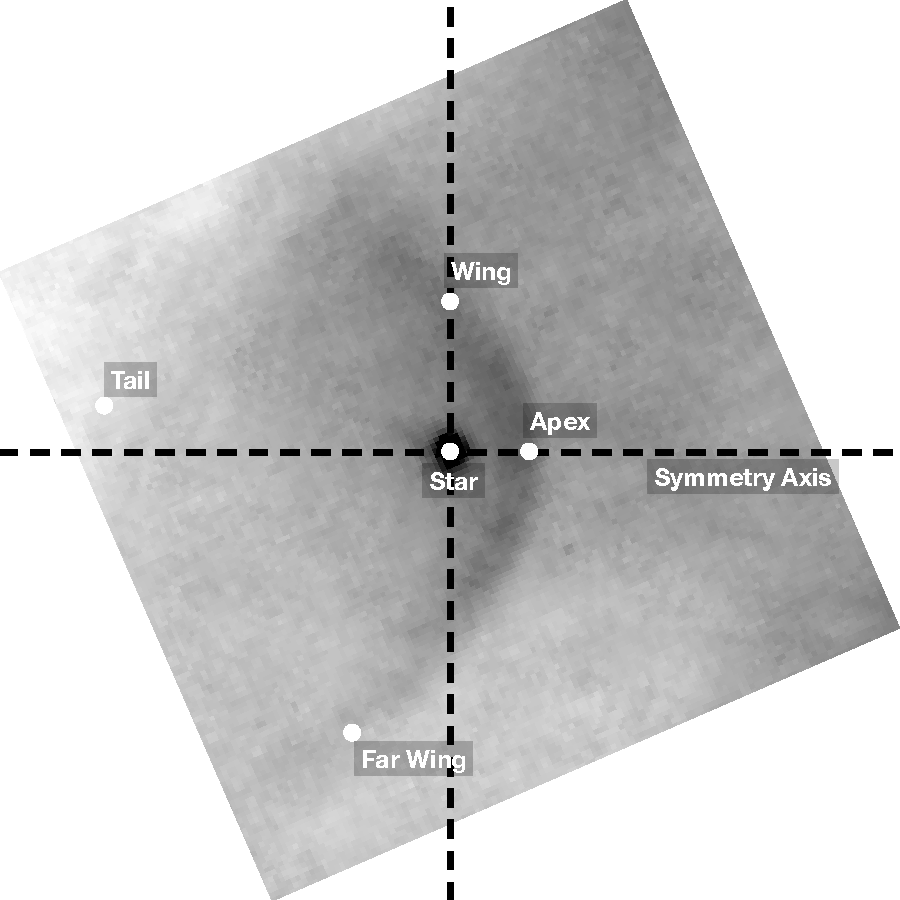
\includegraphics[width=0.5\linewidth]{./Figures/bow-terminology}
  \caption{Terminología de un choque de Proa \textit{estelar}.}
  \label{fig:terminology}
\end{figure}

\section{Proplyds}
Observaciones en mediano infrarrojo y en líneas de emisión de \Ion{H}{\alpha} y [\Ion{O}{III}] \citep{Robberto:2005, Bally:1998, Bally:2000} muestran de manera clara la presencia de arcos que rodean varios proplyds y otros objetos en la ONC cerca y lejos e la región del Trapecio. \citet{Hayward:1994} abre por primera vez la discusión acerca de la naturaleza de estos arcos (enfocándose en la región del Trapecio), sugiriendo que la presión de radiación y el viento estelar de \thC{} interactúan con el flujo de gas proveniente de cada proplyd individual.

\begin{figure}
  \centering
  \begin{tabular}{lr}    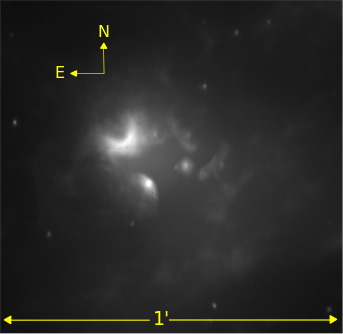
\includegraphics[width=0.5\linewidth]{./Figures/Orion_Robberto}&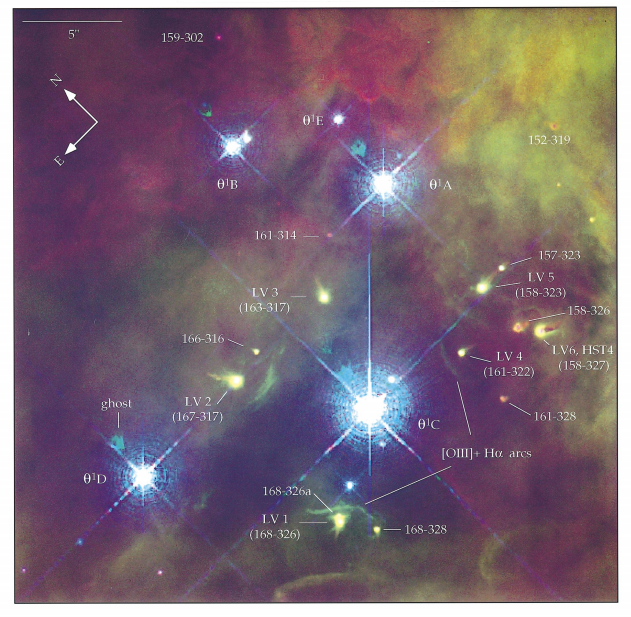
\includegraphics[width=0.5\linewidth]{./Figures/bally-trapezium}
  \end{tabular}
  \caption{Izquierda: La región del trapecio en \SI{10}{\mu m}. \thC{} es la fuente débil al centro de la imagen. Dentro de este campo además se encuentran los proplyds LV1-LV5 con sus respectivos arcos. Al noreste se encuentra una fuente extensa llamada la Nebulosa Ney Allen (NA). El norte es encuentra hacia arriba y el este a la izquierda. El tamaño del campo es de aproximadamente $1' \times 1'$ \citep{Robberto:2005}. Derecha: La región del trapecio en mosaico de colores con imágenes de la Cámara Planetaria de Campo Ancho 2 (WPC2) del ciclo 4 del Telescopio Espacial Hubble (HST). El color rojo corresponde al [\Ion{N}{II}], el verde al \Ion{H}{\alpha} y el azul es [\Ion{O}{III}] \citep{Bally:1998}.}
\end{figure}

Asimismo, en \citet{Robberto:2005} se hicieron mediciones de la forma de estos arcos, utlizando el radio aparente en el ápex $R_0/D$ y el radio perpendicular a éste $R_{90}/D$ (la alatud en este trabajo, excepto que normalizada con la distancia a \thC{} $D$, ver \S \ref{sec:char-rad}) para los proplyds LV1-LV5 y la nebulosa Ney-Allen, y los compararon con el modelo de capa delgada \citep{Canto:1996} (figura \ref{fig:Robberto}). Encontraron que aunque los proplyds LV1, LV4 y posiblemente LV5 ajustan a dicho modelo, pero el resto se aleja mucho de las curvas teóricas. Ésto no se puede atribuir atribuir a las limitaciones de la aproximación algebraica hecha por \citet{Canto:1996}, debido a que aun con todas las simplificaciones que conlleva, ajusta bien con modelos hidrodinámicos más complejos (\citet{Garcia-Arredondo:2001}, figura \ref{fig:GA-simulation}). Este trabajo es en parte la inspiración para esta tesis, ya que para explicar la discrepancia en la figura \ref{fig:Robberto} con los proplyds restantes nos llevó a extender el modelo de \citet{Canto:1996} al caso donde el viento interior no es isotrópico. En la figura \ref{fig:generic-bowshock} se explica el modelo general para explicar éstos choques de proa: el flujo fotoevaporado de un proplyd, ya sea isotrópico o anisotrópico, interactúa con el viento estelar de \thC{}, formando dos choques separados por una discontinuidad de contacto. El Frente de Ionización del proplyd es tipo D (ver \S \ref{sec:photoevaporation}), por lo que la velocidad del flujo fotoevaporado es cercano a la velocidad del Sonido y se acelera máximo hasta $M\sim 3$, y su densidad electrónica es de $n_e\sim \SI{e6}{cm^{-3}}$ (ver \S \ref{sec:prop-Johnstone}). Por otro lado, el viento de \thC{} ha alcanzdo su velocidad terminal, que es de $M > 100$ con una tasa de pérdida de masa de $\dot{M} \simeq \SI{4e-7}{M_\odot.yr^{-1}}$ \citep{Gagne:2005}. Bajo estas condiciones, el choque exterior es poco denso y extenso y el choque interior es más denso y angosto. Por tanto, el enfriamiento en el choque interior es más eficiente y consideramos que este choque es radiativo mientras que el choque exterior no.

\begin{figure}
  \centering
  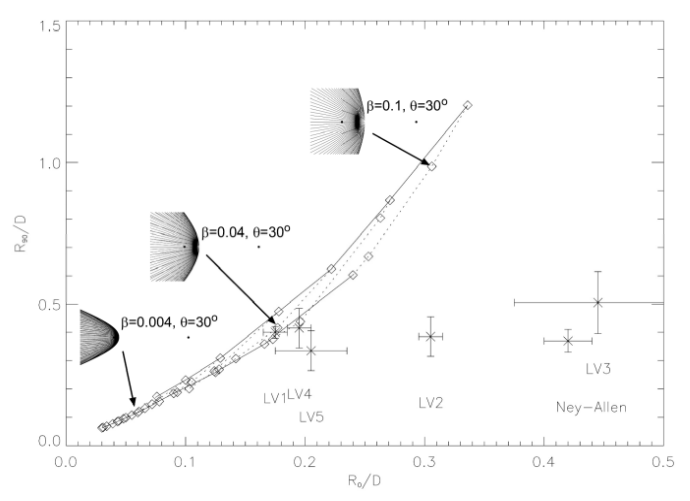
\includegraphics[width=0.7\linewidth]{./Figures/robberto}
  \caption{Comparación de los Radio Característicos aparentes $R'_{90}/D$ y $R_0/D$ para los proplyds LV1-LV5 y para la Nebulosa Ney-Allen mostrados con puntos y sus respectivas incertidumbres, y los diamantes abiertos se muestran soluciones al modelo de capa delgada de \citep{Canto:1996} para $\beta=[0.001, 0.002, 0.004, 0.01, 0.02, 0.1]$ y para intervalos de inclinaciones de $15^\circ$ entre $0^\circ$ y la inclinación máxima (ver \S \ref{sec:fundamental-parameters}, \ref{sec:projection}).}
  \label{fig:Robberto}
\end{figure}

\begin{figure}
  \centering
  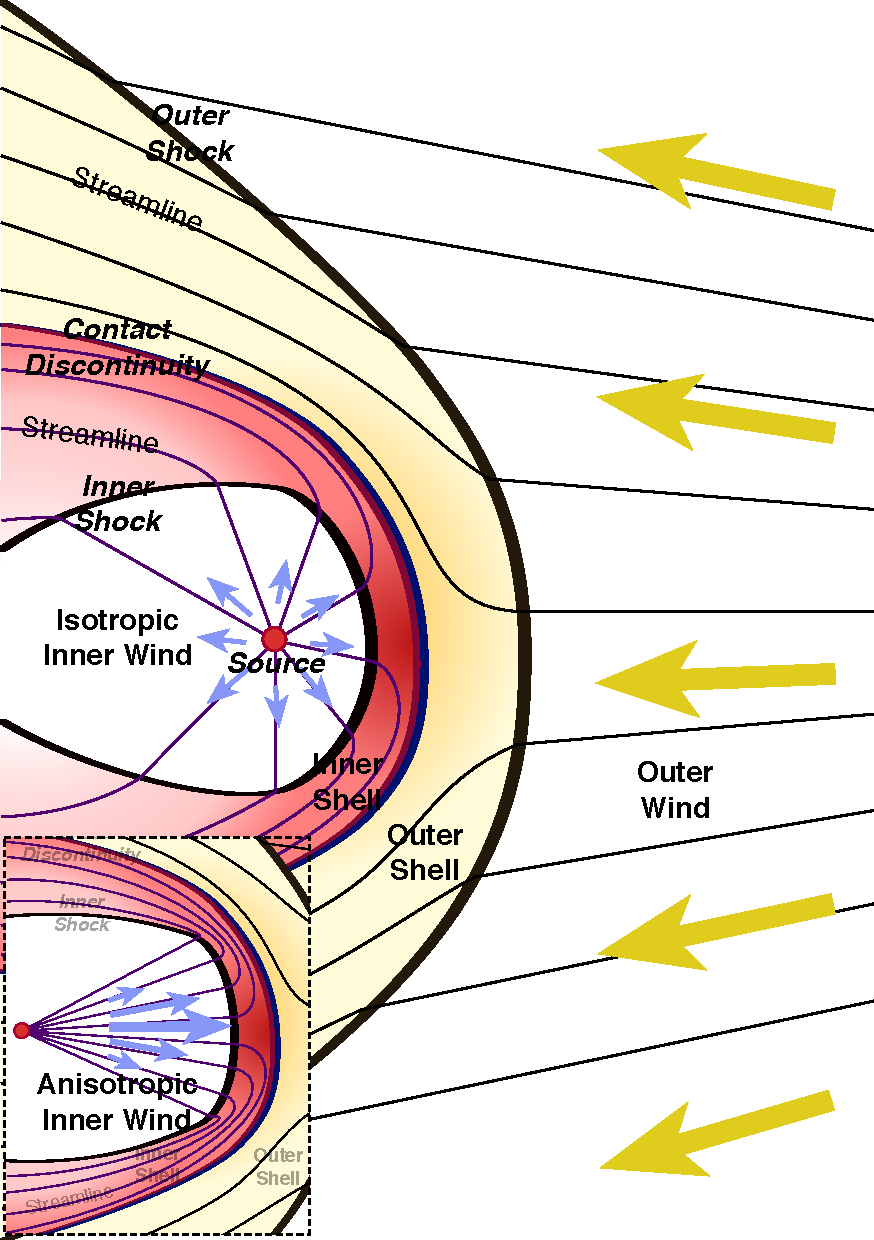
\includegraphics[width=0.7\linewidth]{./Figures/generic-bowshock}
  \caption{Esquema del choque de proa de un proplyd: el viento rápido proveniente de una estrella masiva interactúa con el flujo fotoevaporado de un proplyd que puede ser isotrópico o anisotrópico. Se forman dos choques separados por una discontinuidad de contacto, y dependiendo de la velocidad y densidad de los vientos, dichos choques pueden ser radiativo o no. En el caso de los proplyds más cercanos al trapecio, solo el choque interno es radiativo.}
  \label{fig:generic-bowshock}
\end{figure}


\begin{figure}
  \centering
  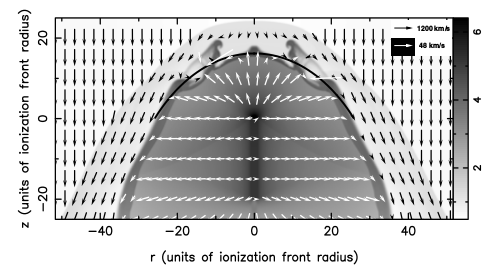
\includegraphics[width=0.7\linewidth]{./Figures/GA-simulation}
  \caption{Resultado de una simulación hidrodinámica de la interacción de un flujo fotoevaporado de un proplyd con un viento estelar. Las flechas indican la velocidad de los flujos (negro para el viento estelar y blanco para el flujo fotoevaporado del proplyd) y la escala gris representa el logaritmo de la densidad. Los ejes están en coordenadas cilíndricas $(r, z)$ en unidades del radio del IF. El arco negro representa la solución analítica de la posición de la discontinuidad de contacto de un choque ancantoide con $k=1/2$ y $\beta=0.002$ \citep{Garcia-Arredondo:2001}}
  \label{fig:GA-simulation}
\end{figure}

\section[Objetos LL]{Choques de Proa ``In Situ'': Objetos LL'}
\label{sec:Luis-LL}

El arquetipo de esta clase de objetos es LL\,Ori (LL1 de aquí en adelante), son llamados también choques ``in situ'' \citep{Kobulnicky:2016}, donde el choque se da cuando viento de una estrella interactúa con un flujo tal como un flujo de champaña. Sin embargo, no es del todo claro el tipo de flujo interno proveniente de la estrell central (figura \ref{fig:LL-scheme}). \citet{Gutierrez-Soto:2015a} hizo un catálogo de objetos dentro de ONC en los que se observan choques de proa, algunos de ellos no habían sido identificados previamente, a la vez que se realizaron mediciones de $(R'_0, R'_c)$ de cada objeto (ver \S \ref{sec:fundamental-parameters}, \ref{sec:projection}). En la figura \ref{fig:Luis-mosaic-1} mostramos algunos ejemplos de este catálogo. A diferencia de los choques de proa más próximos a \thC{}, los objetos LL pueden presentar dos cáscaras. Si ese es el caso, los radios $(R'_0, R'_c)$ fueron medidos para ambas cáscaras, así como el grosor $H'$ que es la diferencia de $R'_0$ de ambas cáscaras y la orientación (figura \ref{fig:methodology-LL}).

\begin{figure}
  \centering
  \includegraphics[width=\linewidth]{./Figures/LL-outer-inner-extend-Luis}
  \caption{Posibiles escenarios para los flujos en interacción de los choques de proa en ONC. Izquierda: Un flujo de champaña transónico interactúa ya sea con el flujo fotoevaporado de un proplyd o con un viento estelar, este caso aplica para los arcos más alejados de \thC{}. Derecha: El viento estelar proveniente de una estrella tipo O interactúa con el flujo fotoevaporado de un proplyd. Aplica para los proplyds más cercanos a \thC{}.}
  \label{fig:LL-scheme}
\end{figure}

\begin{figure}
  \centering
  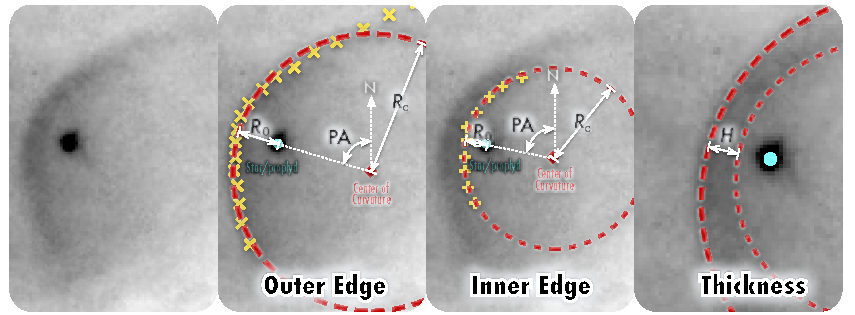
\includegraphics[width=0.7\linewidth]{./Figures/radius-methodology-Luis}
  \caption{Metodología para la medición de los radios característicos $(R'_0, R'_c)$. Para un arco dado, se traza la posición de las dos cáscaras utilizando marcas con el programa DS9 para imágenes astronómicas (las cruces en la figura). Posteriormente, con un ajuste de mínimos cuadrados se ajusta un círculo a las marcas de cada cáscara para obtener el radio de curvatura aparente $R'_c$ (línea roja rayada). $R'_0$ se obtiene como la distancia mínima entre la posición de la estrella y el ajuste circular y por último el grosor $H'$ se obtiene como la diferencia entre ambas mediciones de $R'_0$, suponiendo que estén disponibles.}
  \label{fig:methodology-LL}
\end{figure}

\begin{figure}
  \centering
  \begin{tabular}{cc}
    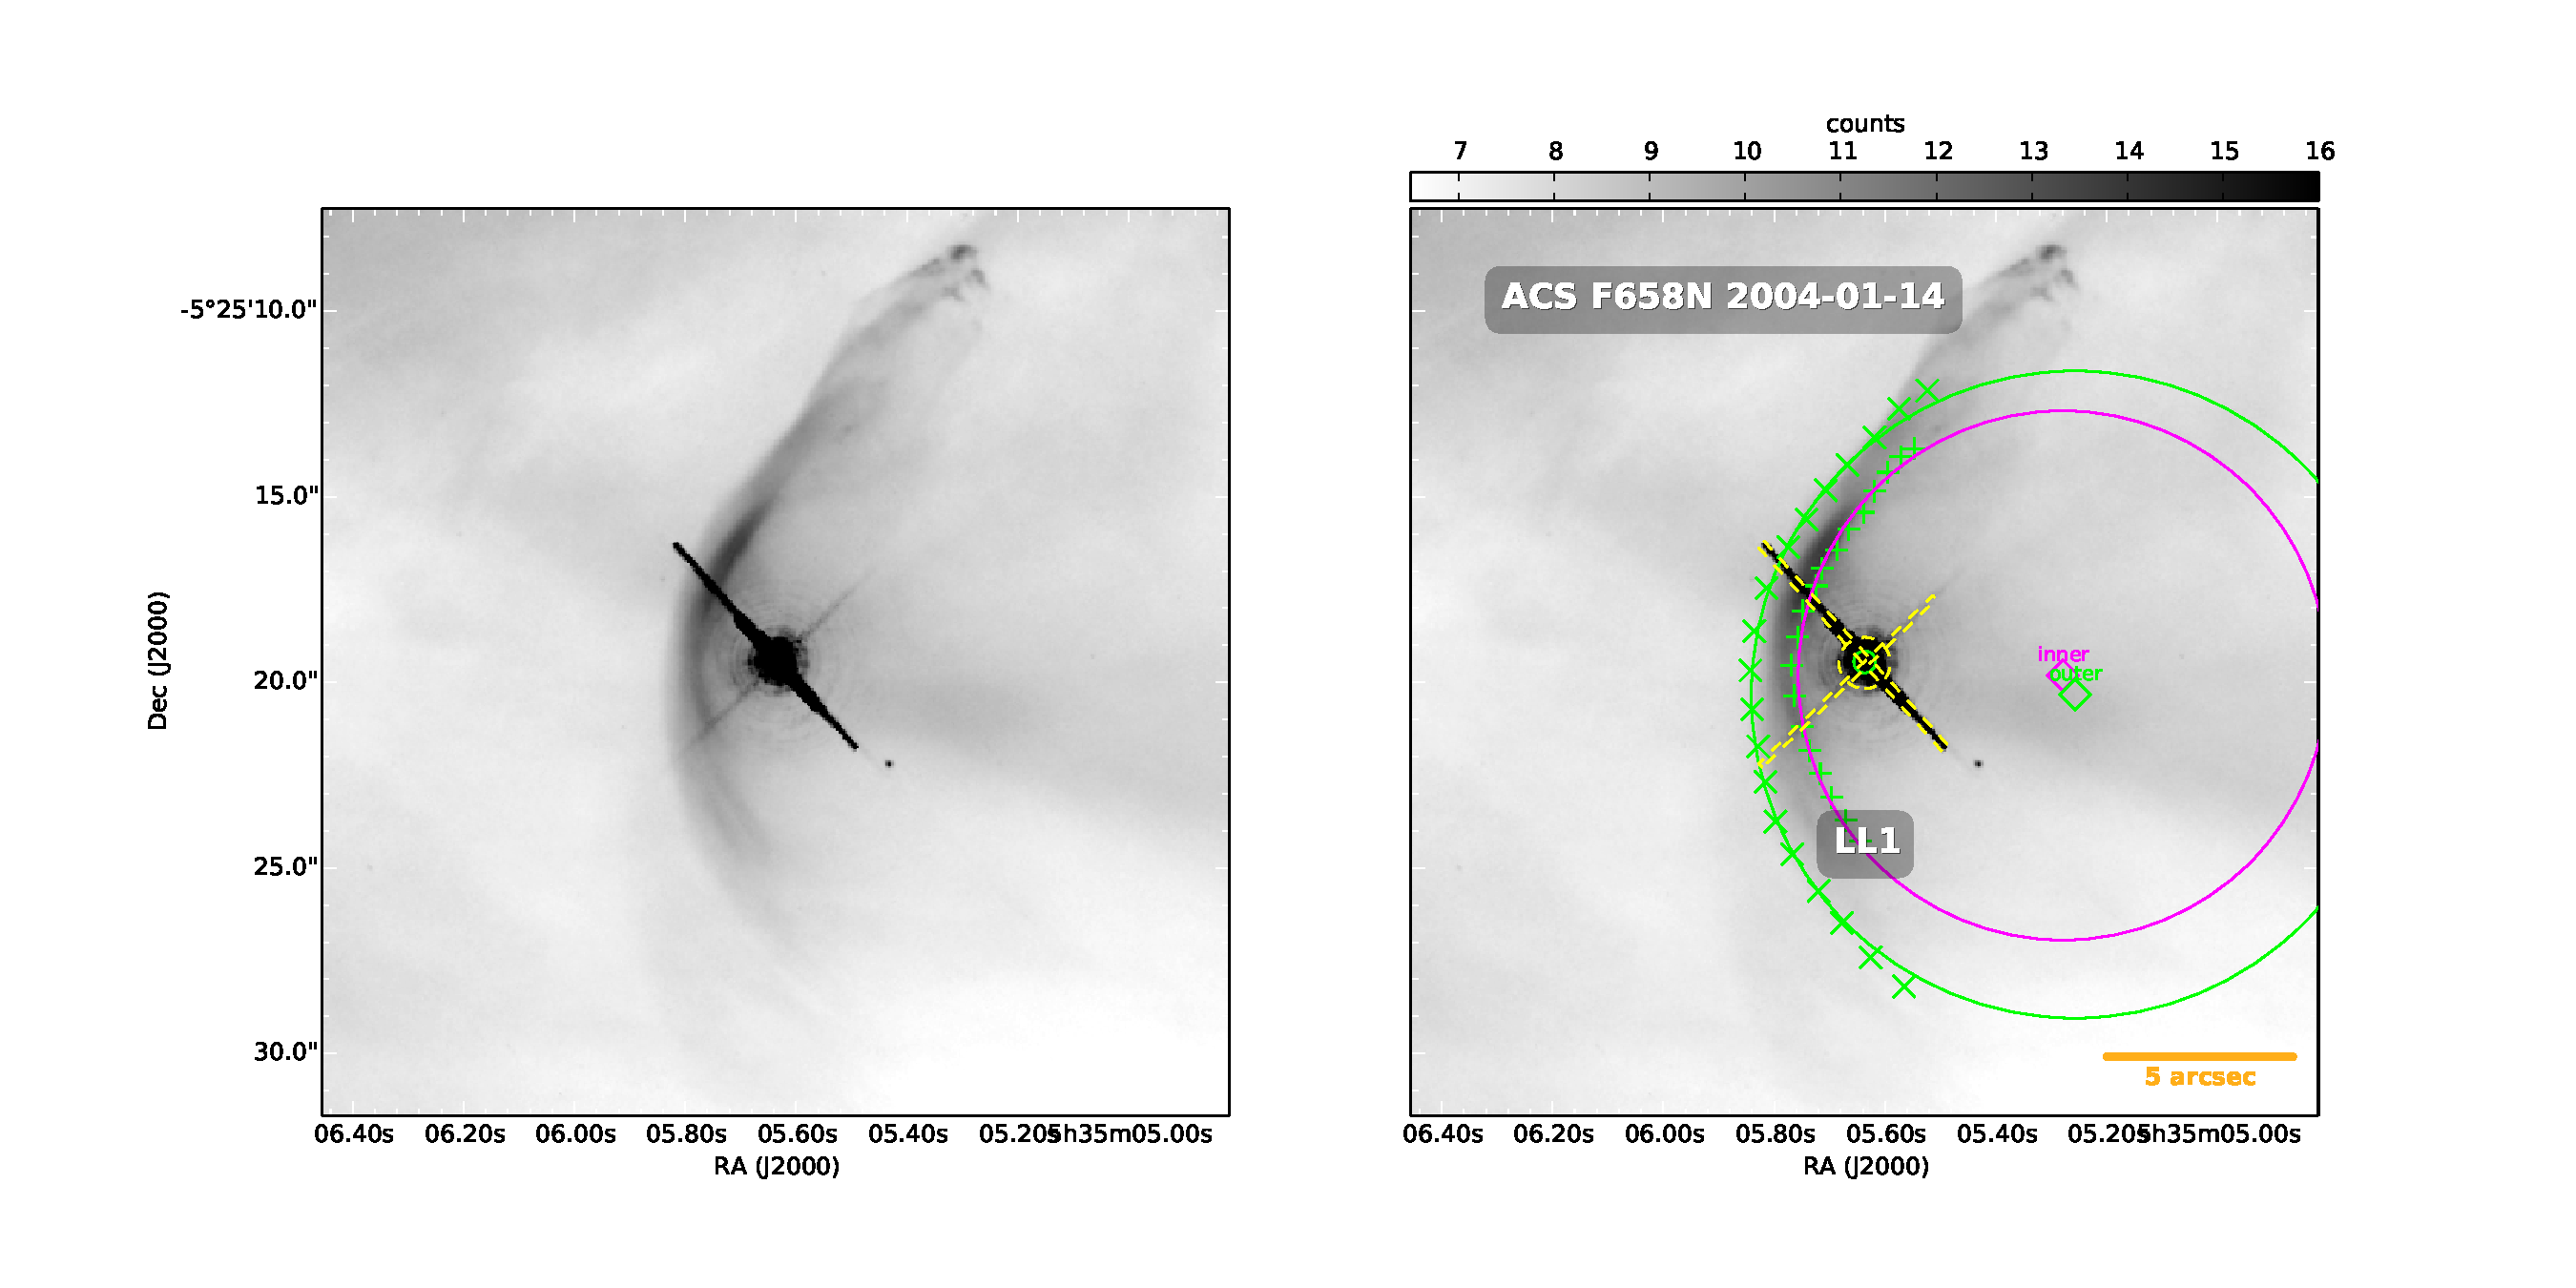
\includegraphics[width=0.5\linewidth]{./Figures/LL1-Bally_01-images} & 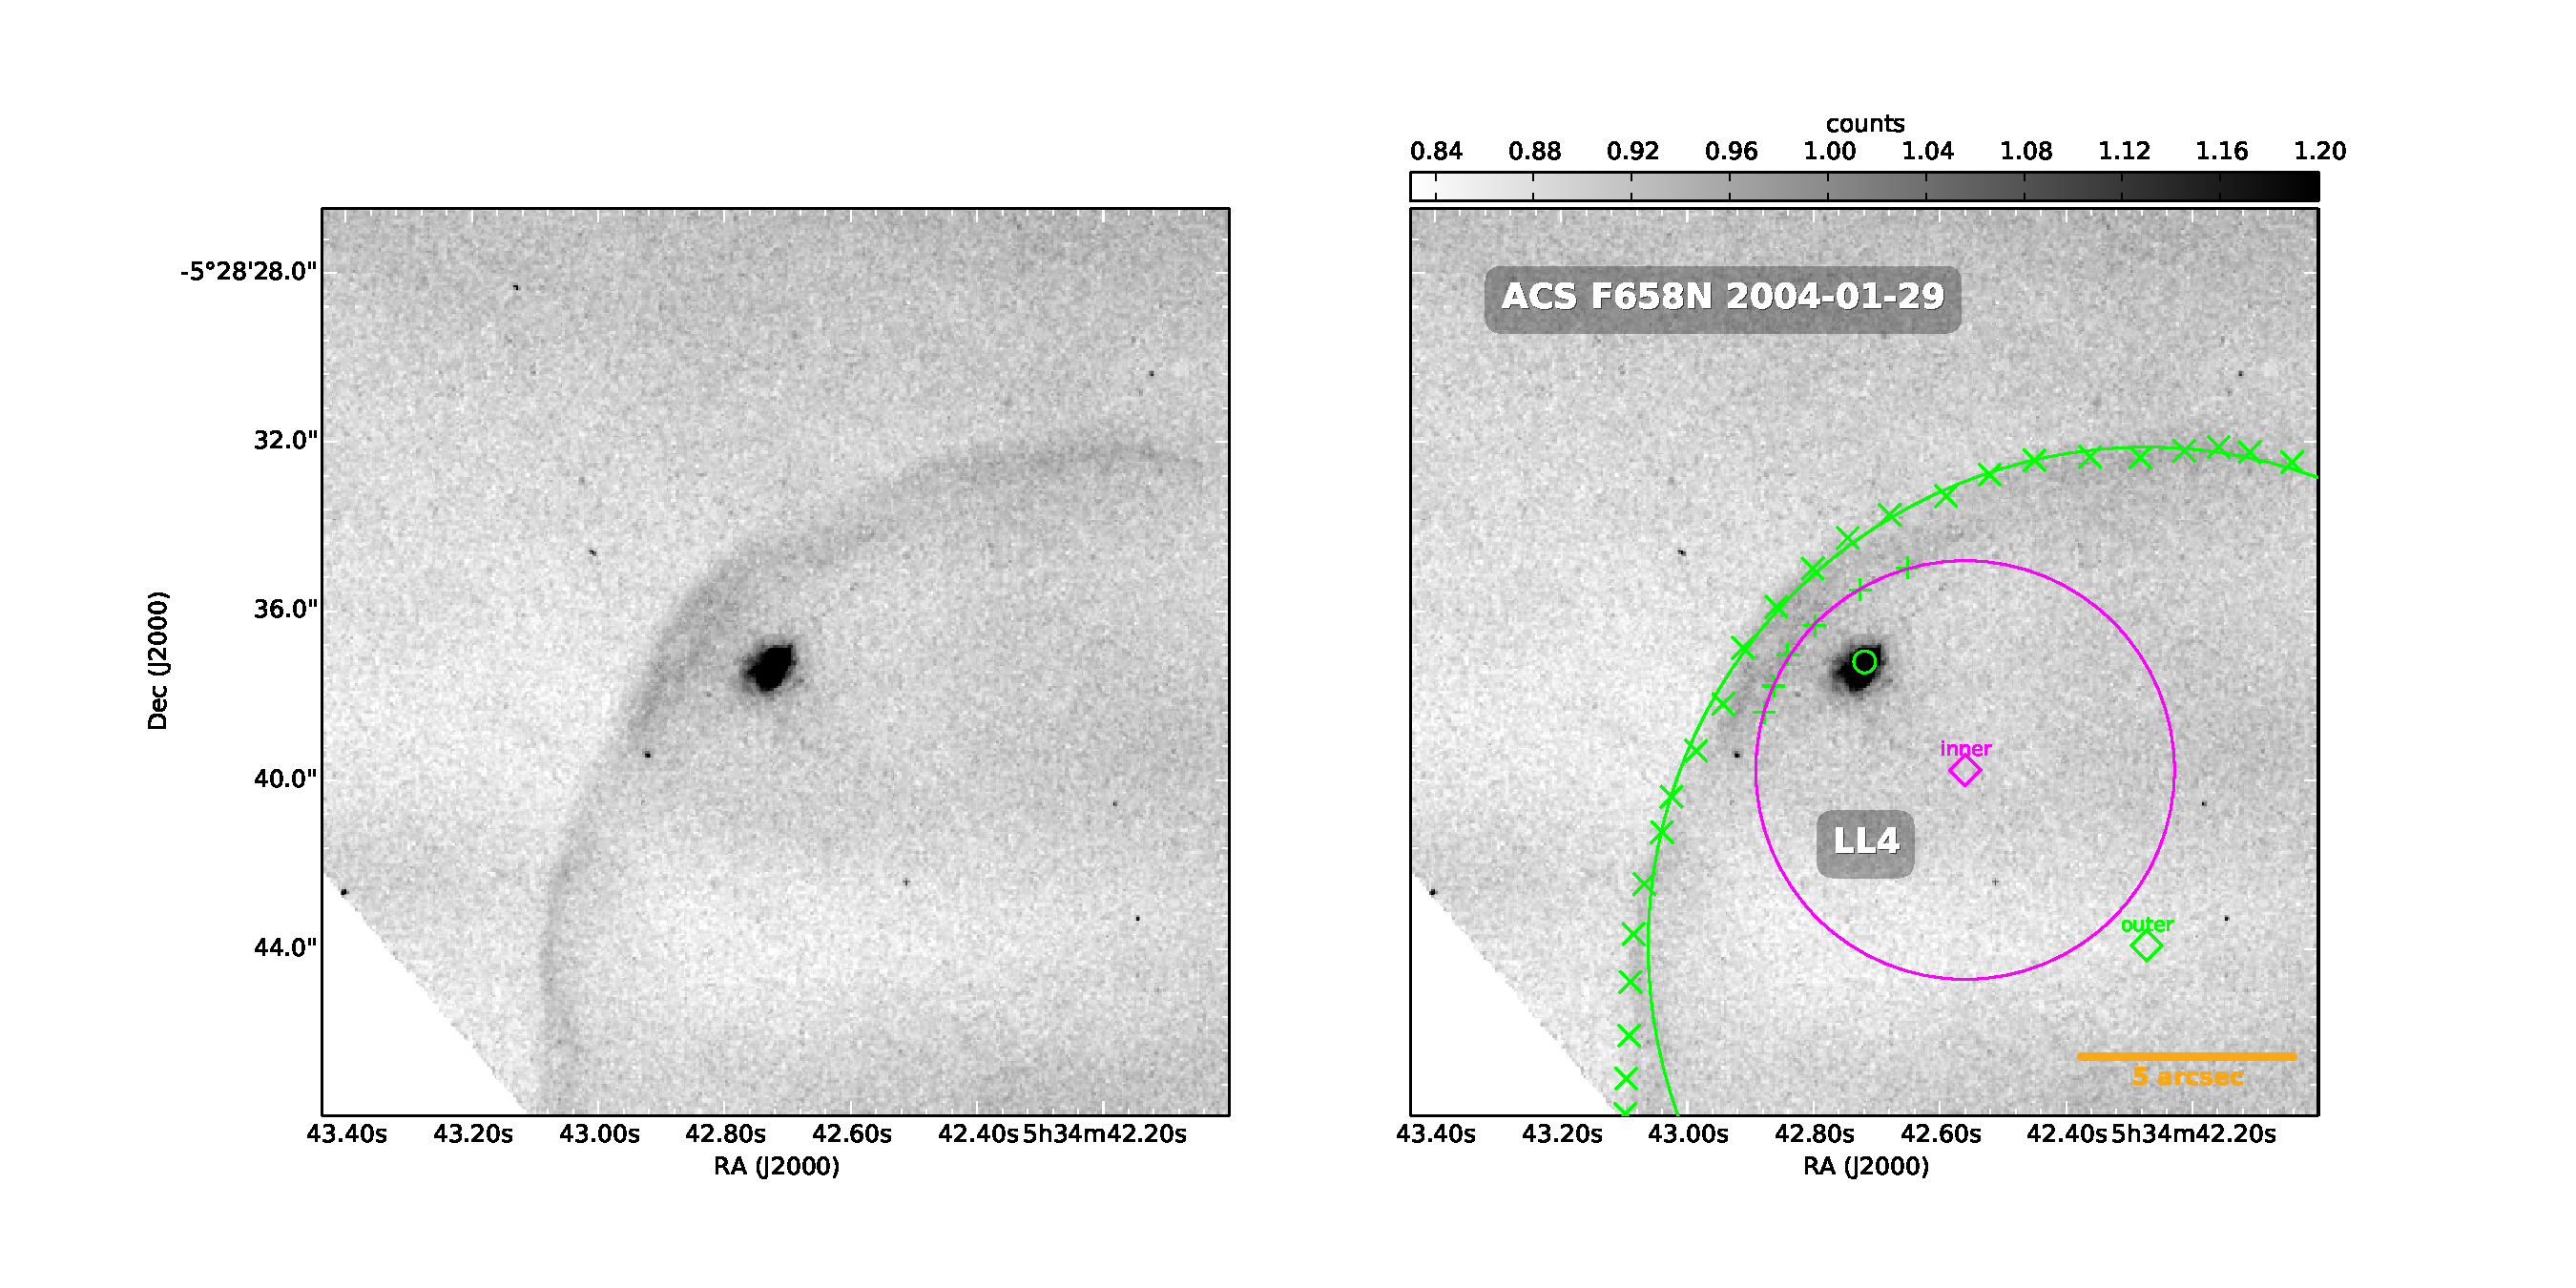
\includegraphics[width=0.5\linewidth]{./Figures/LL4-Bally_24-images} \\ 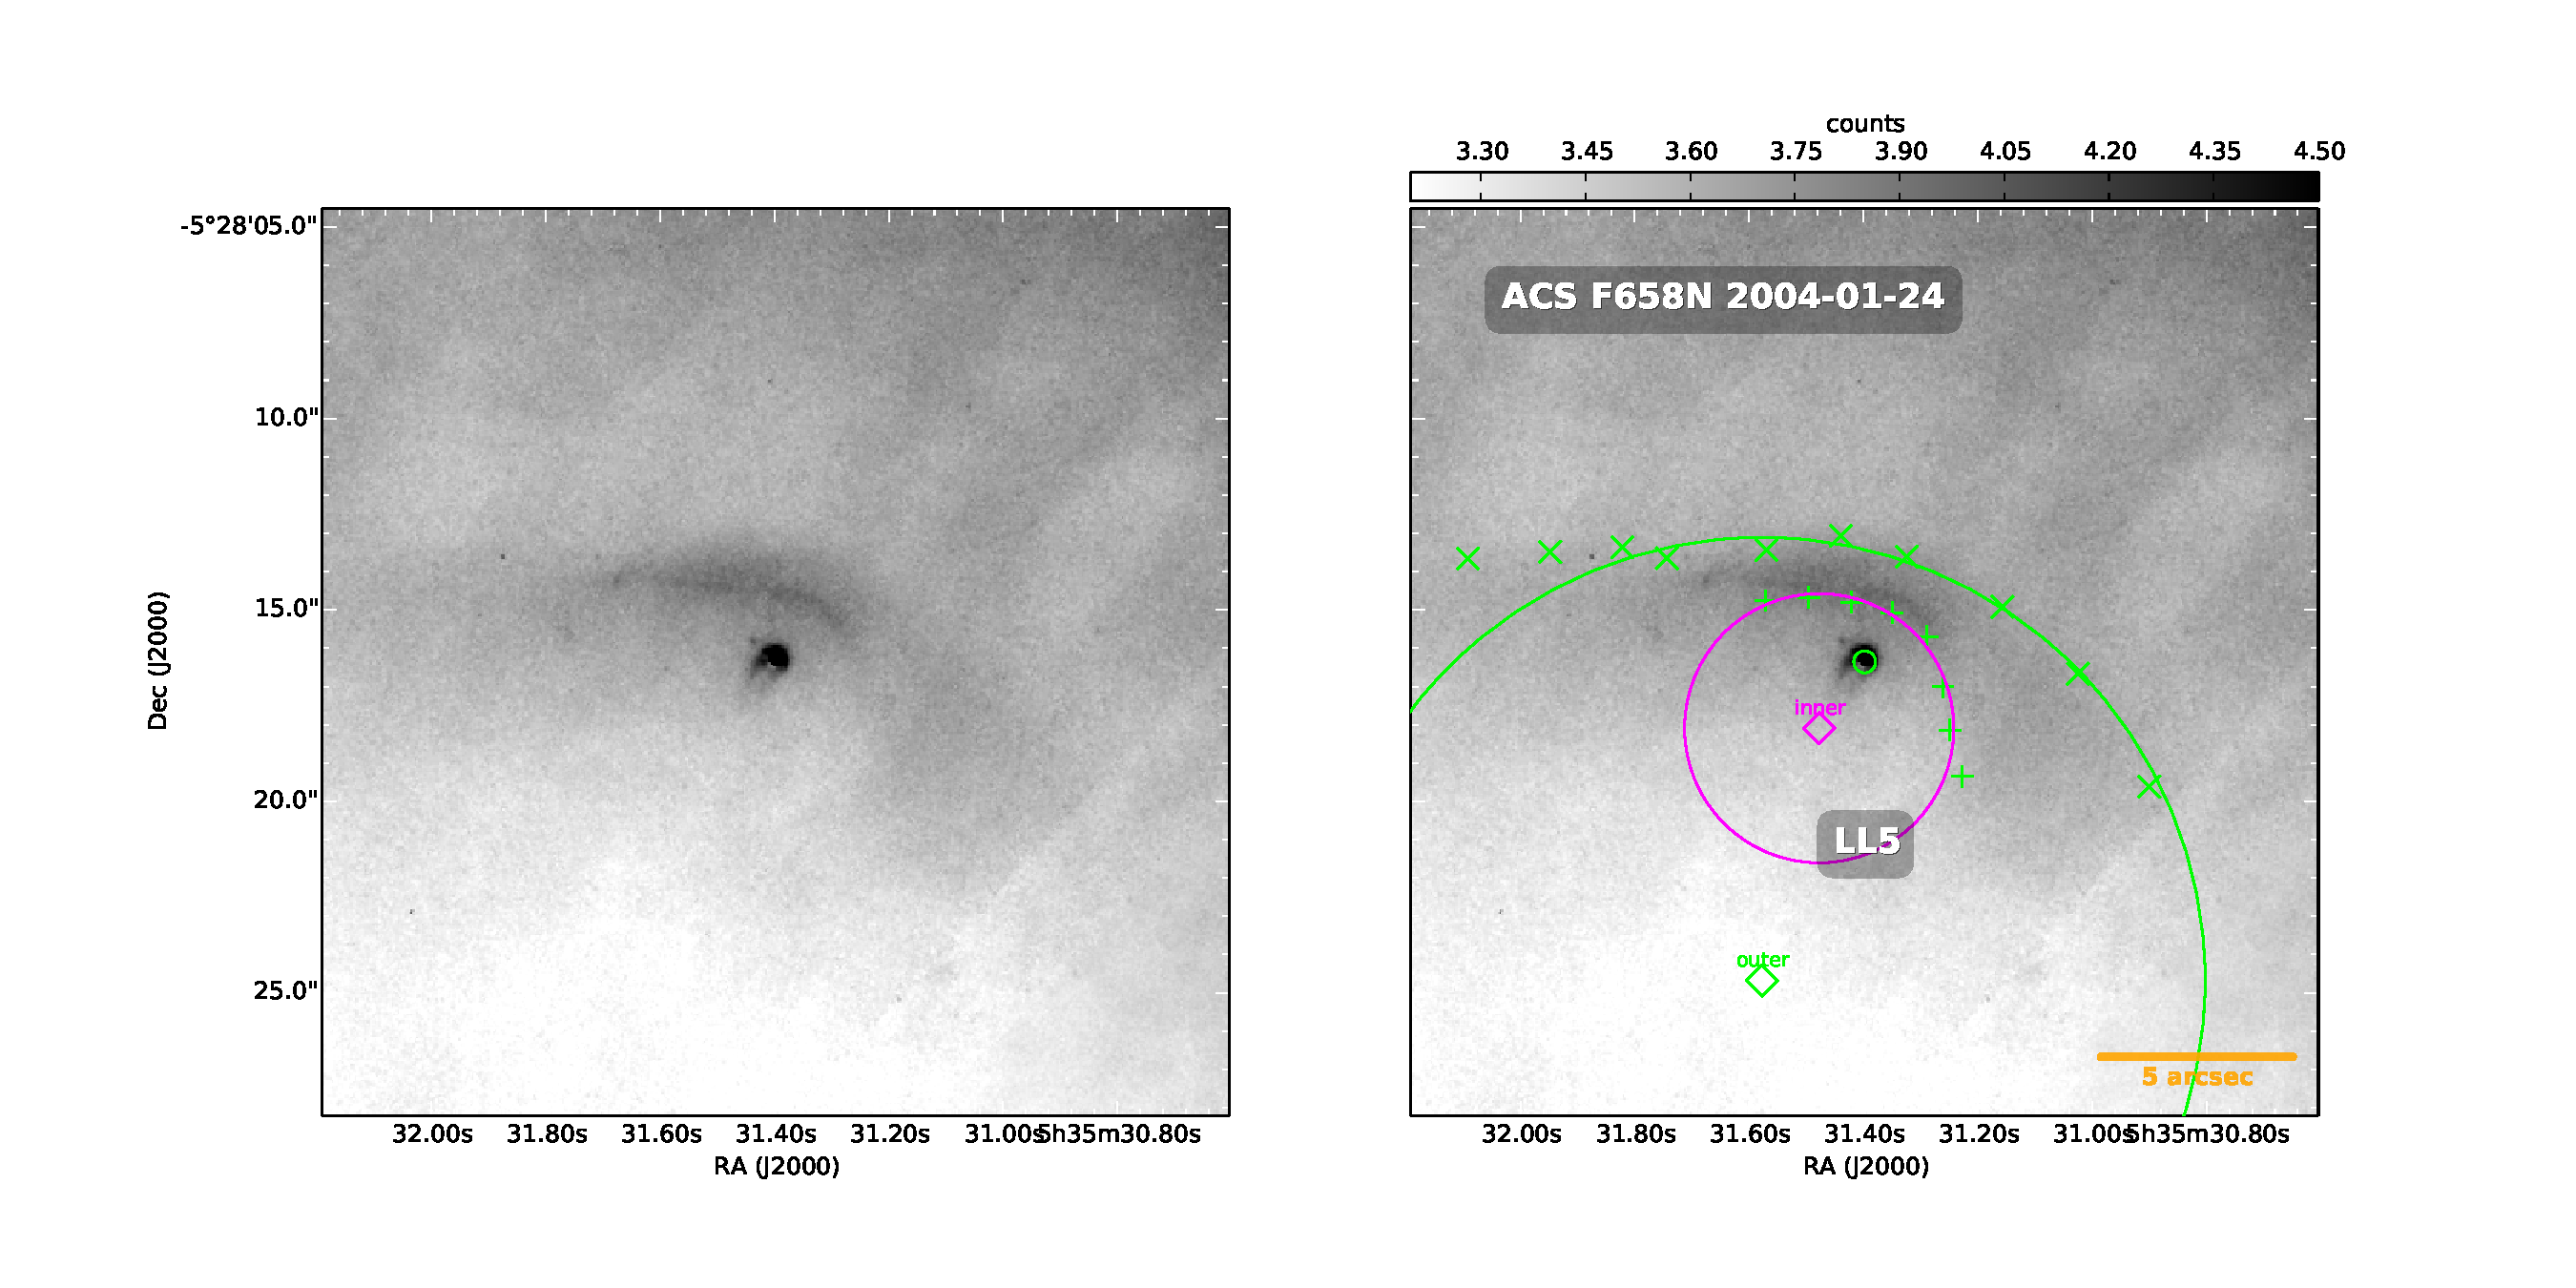
\includegraphics[width=0.5\linewidth]{./Figures/LL5-Bally_07-images} &
    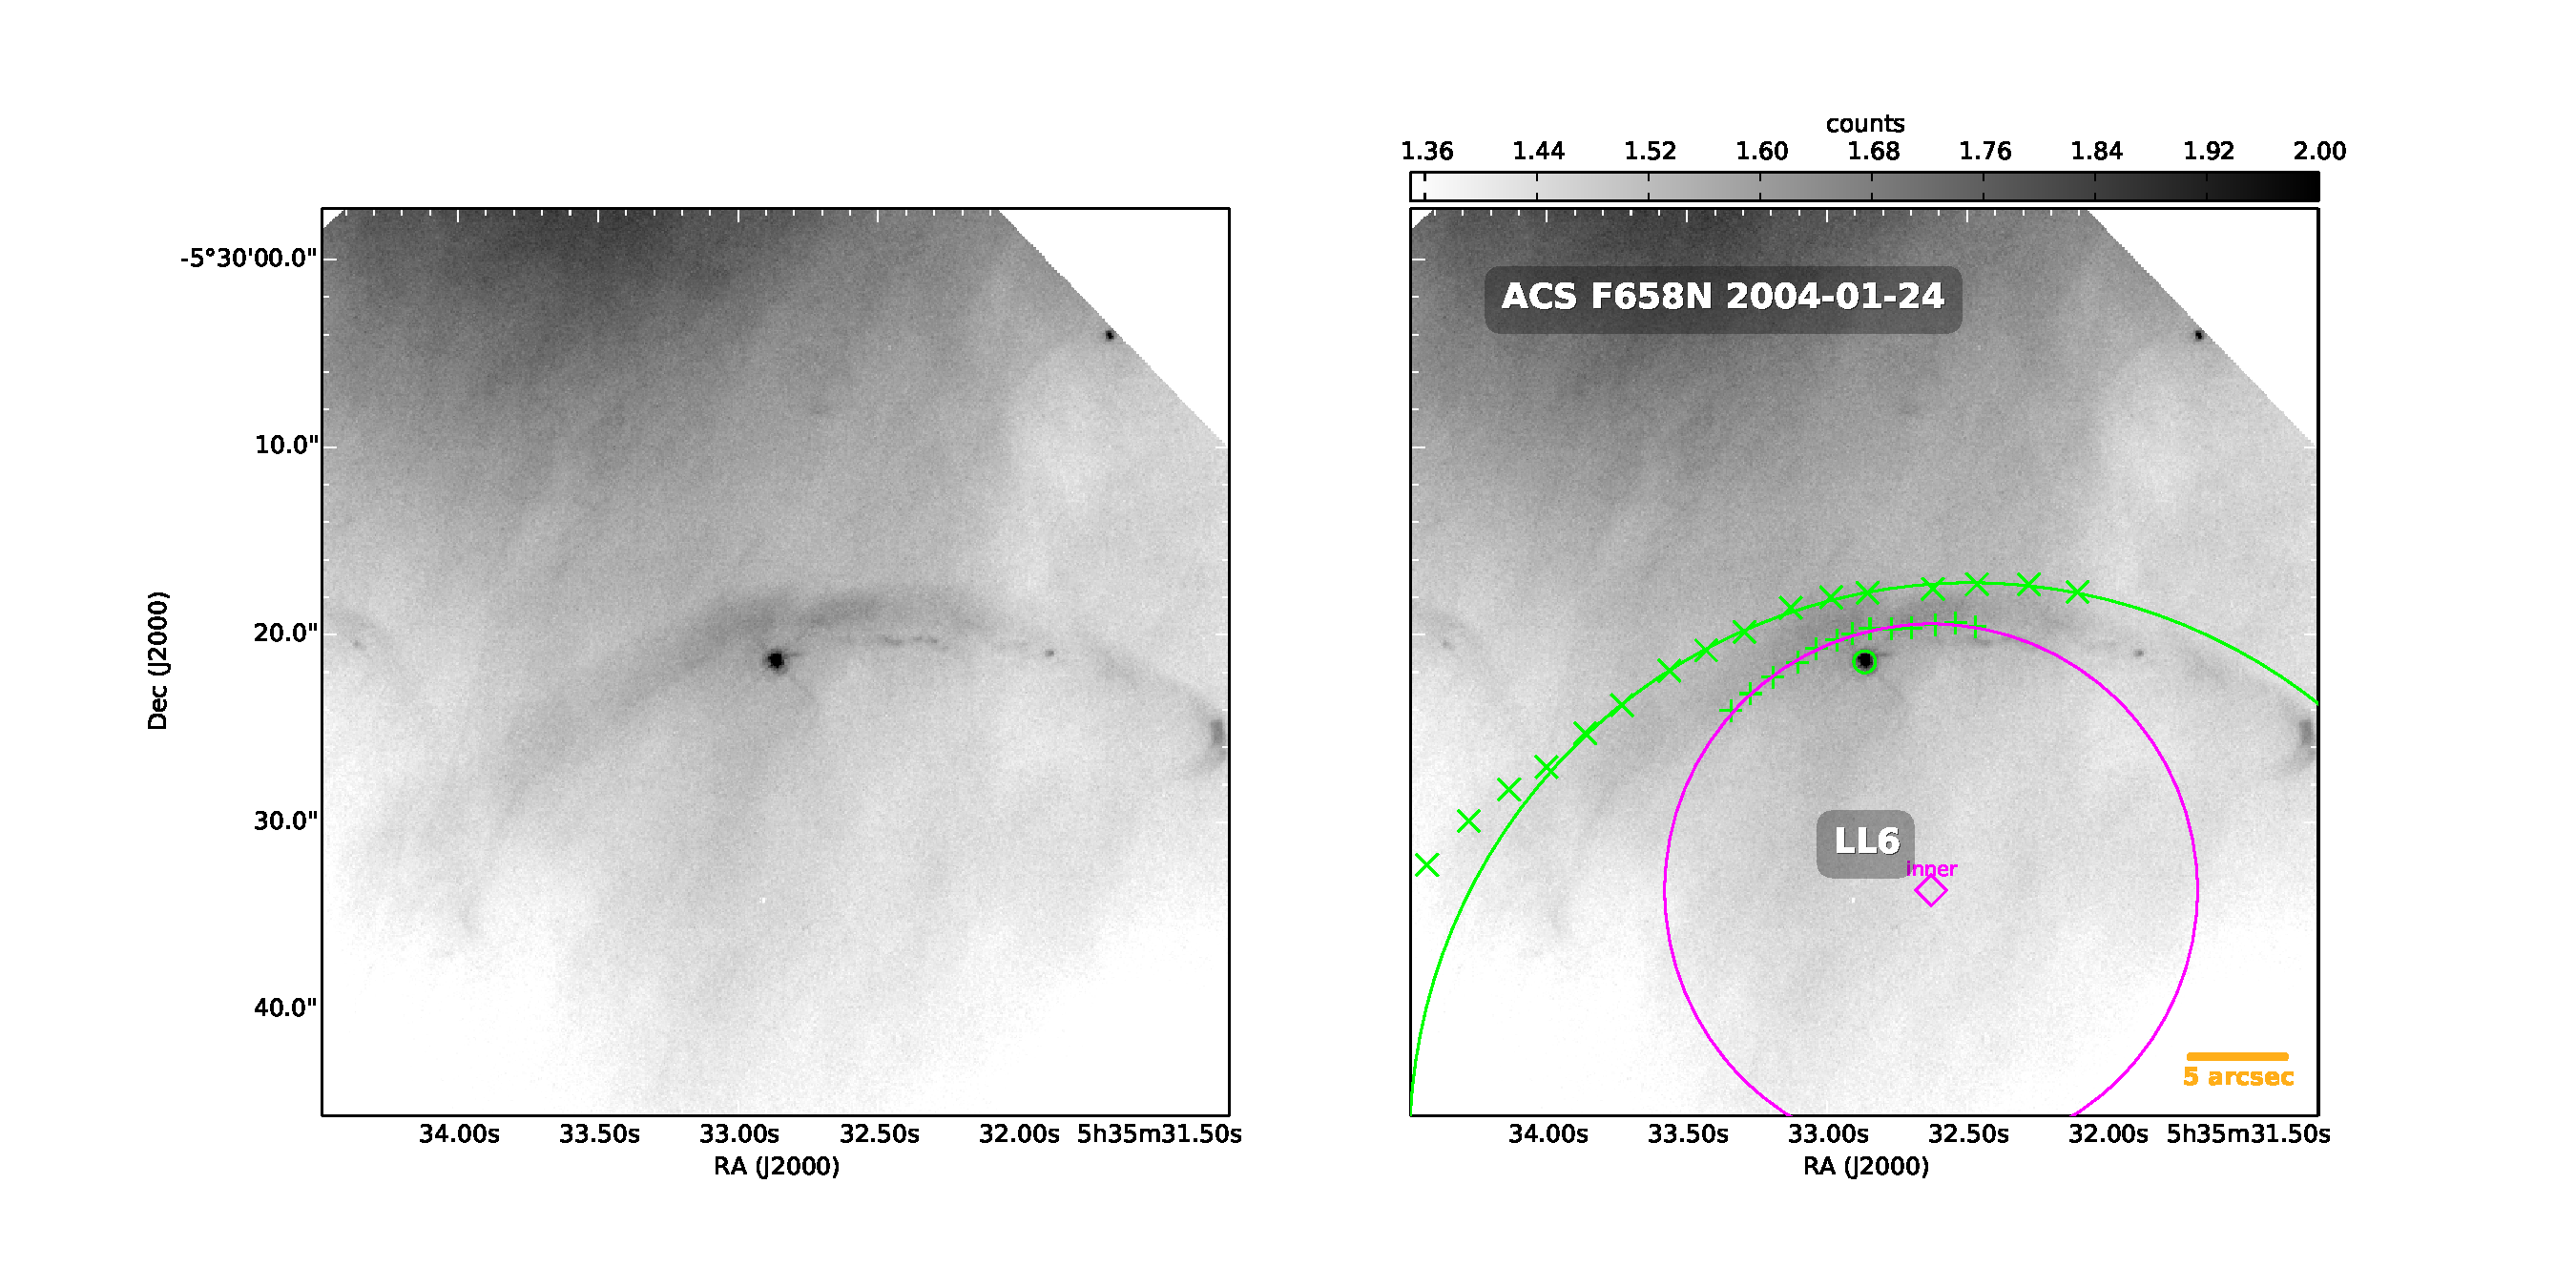
\includegraphics[width=0.5\linewidth]{./Figures/LL6-Bally_08-images} \\ 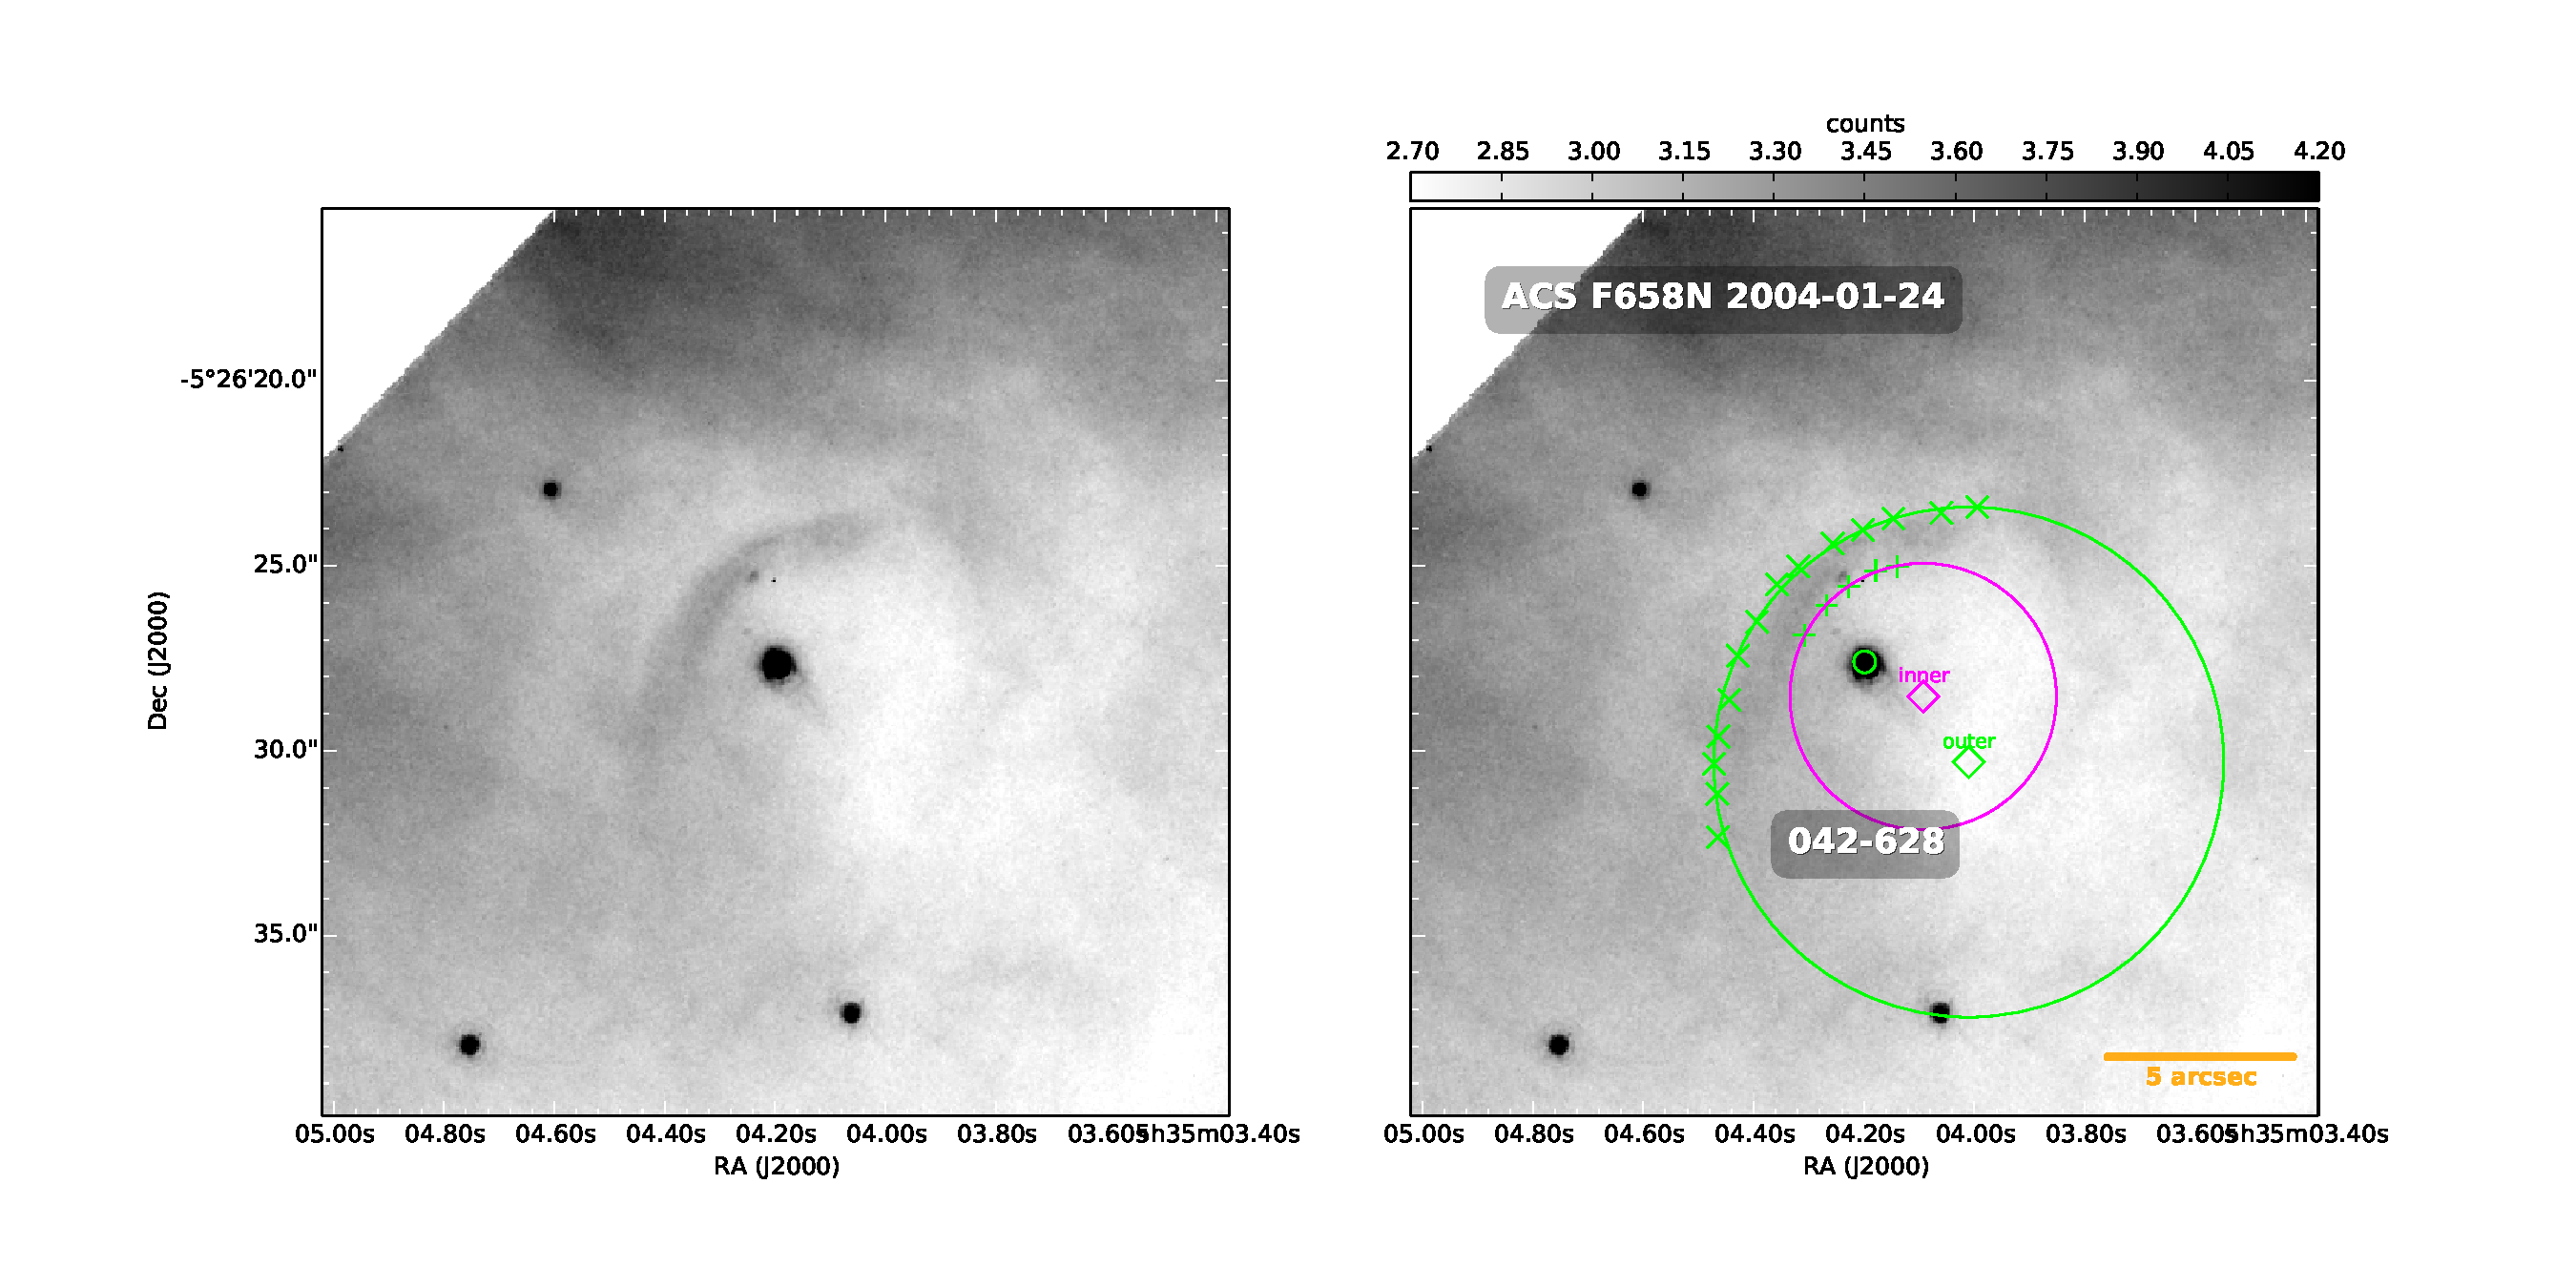
\includegraphics[width=0.5\linewidth]{./Figures/042-628-Bally_16-images} & 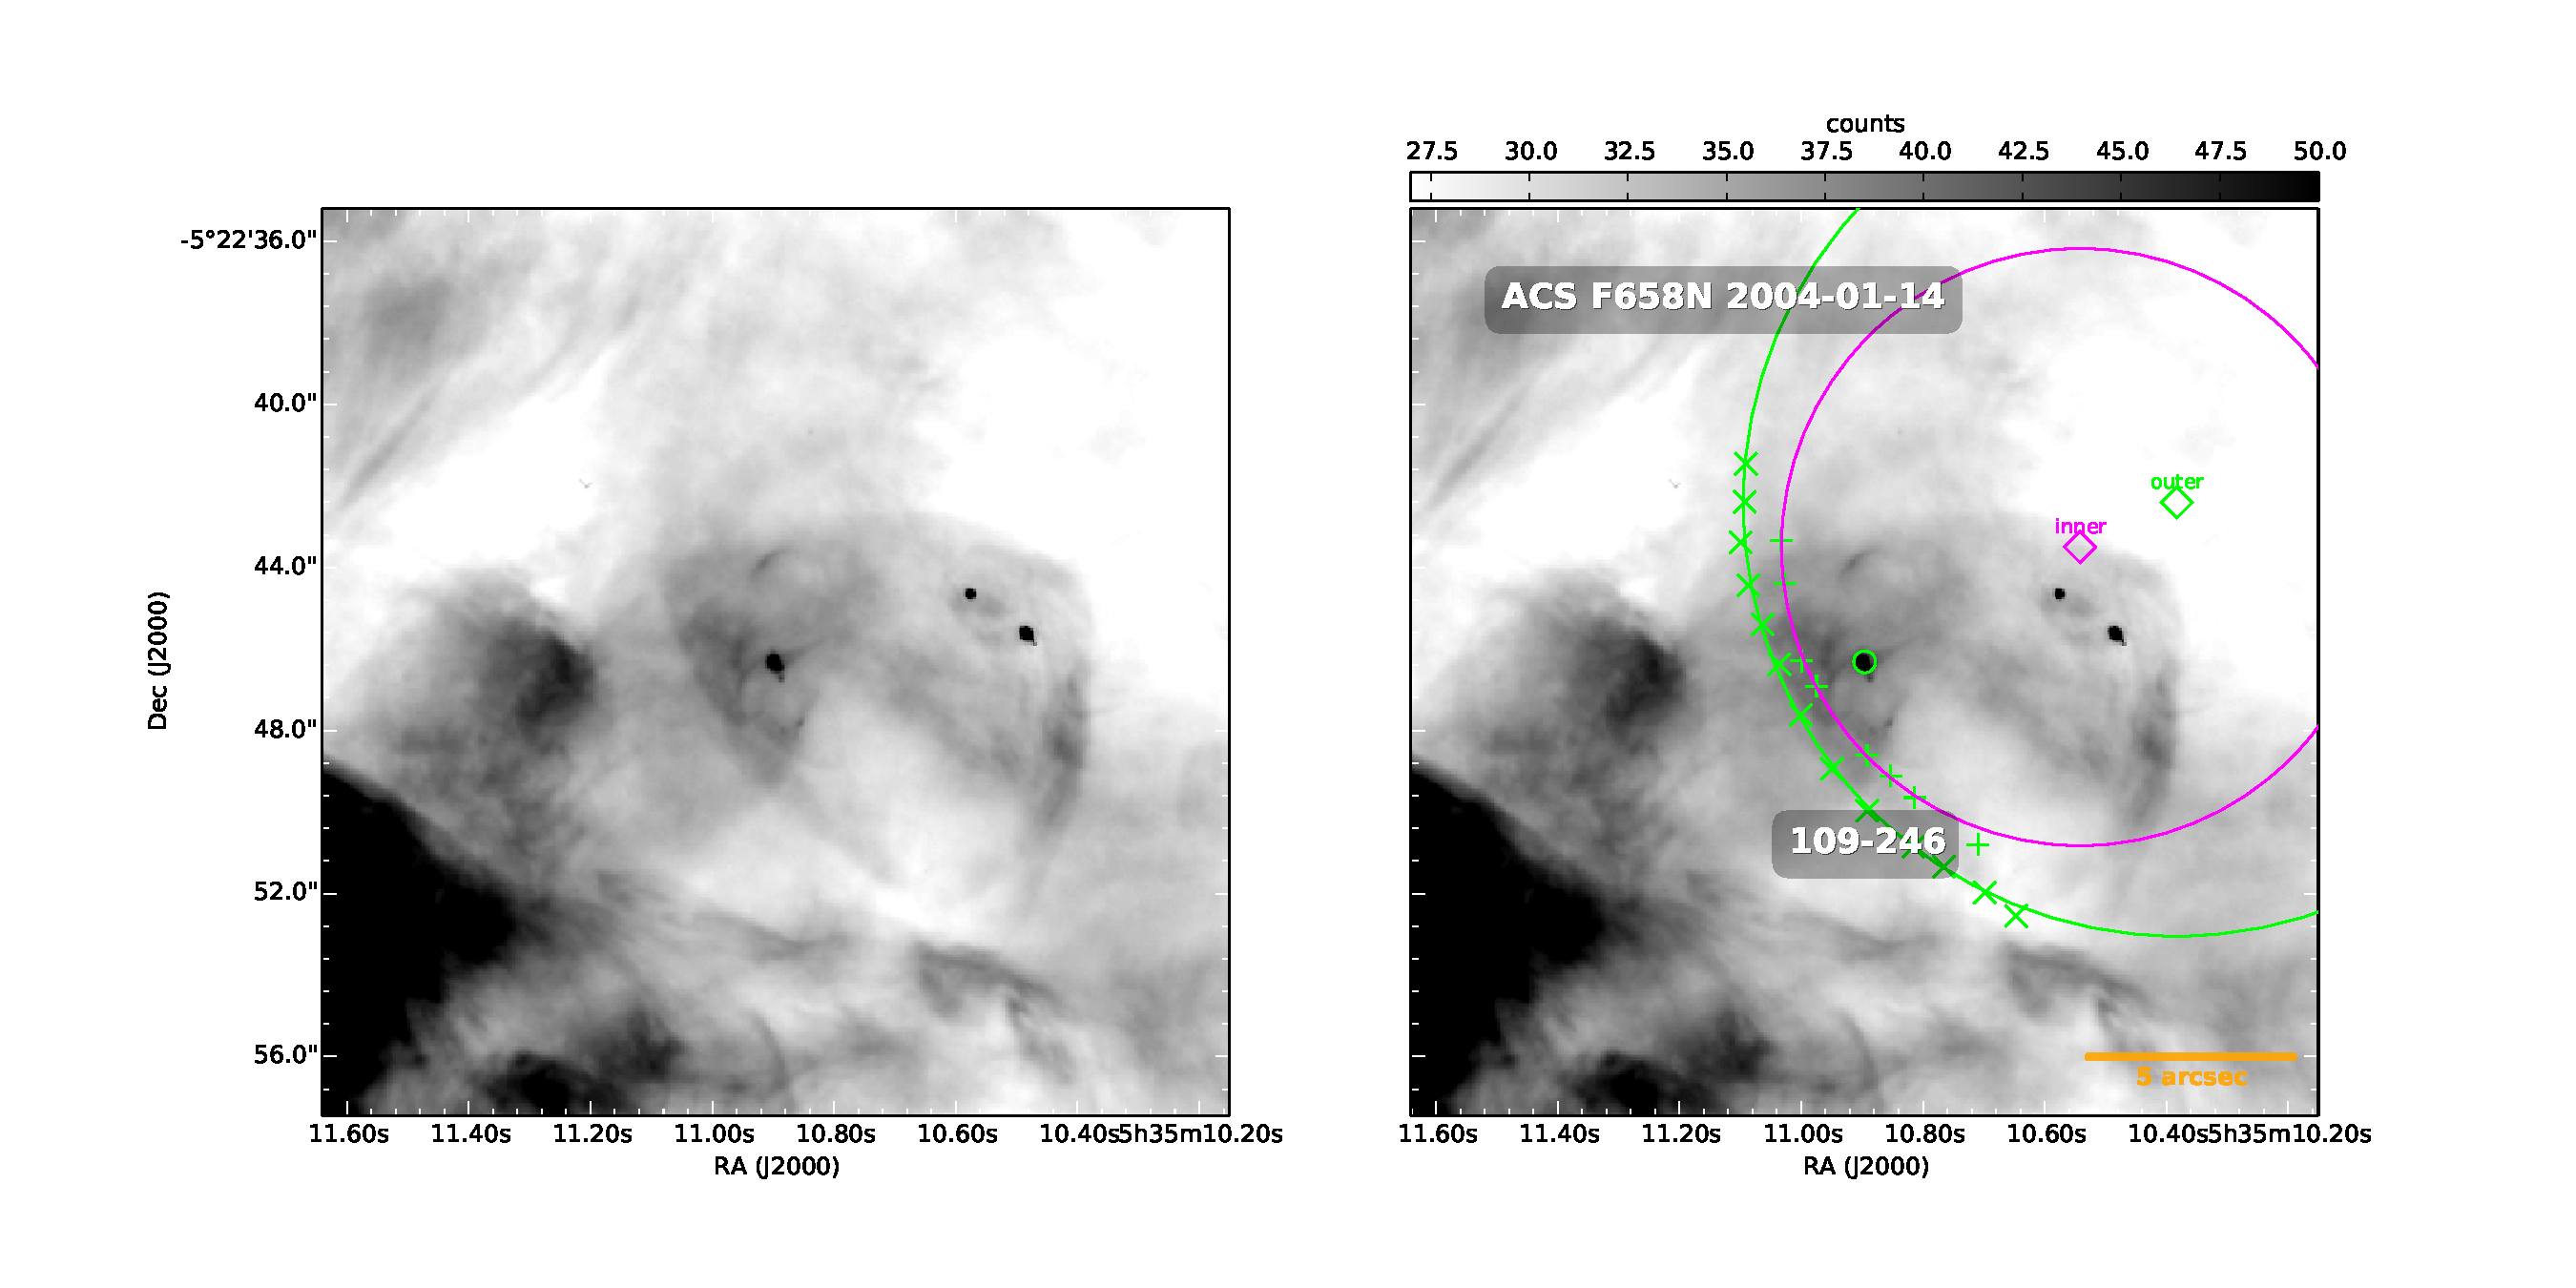
\includegraphics[width=0.5\linewidth]{./Figures/109-246-Bally_01-images} 
  \end{tabular}
  \caption{Ejemplos de objetos LL obtenidos del catálogo de \citet{Gutierrez-Soto:2015a}. A la derecha de cada panel se observa el objeto con las mediciones superpuestas de los radios característicos $(R'_0, R'_c)$ para las cáscaras exterior e interior o solo para una dependiendo del objeto. La escala de grises muestra el brillo, la barra amarilla indica la escala del objeto y las etiquetas mestran el nombre del objeto, el instrumento que se utilizó para obtener la imagen y la fecha en que se obtuvo.}
  \label{fig:Luis-mosaic-1}
\end{figure}


\begin{figure}
  \centering
  \ContinuedFloat
    \captionsetup{list=off,format=cont}
  \begin{tabular}{cc}
    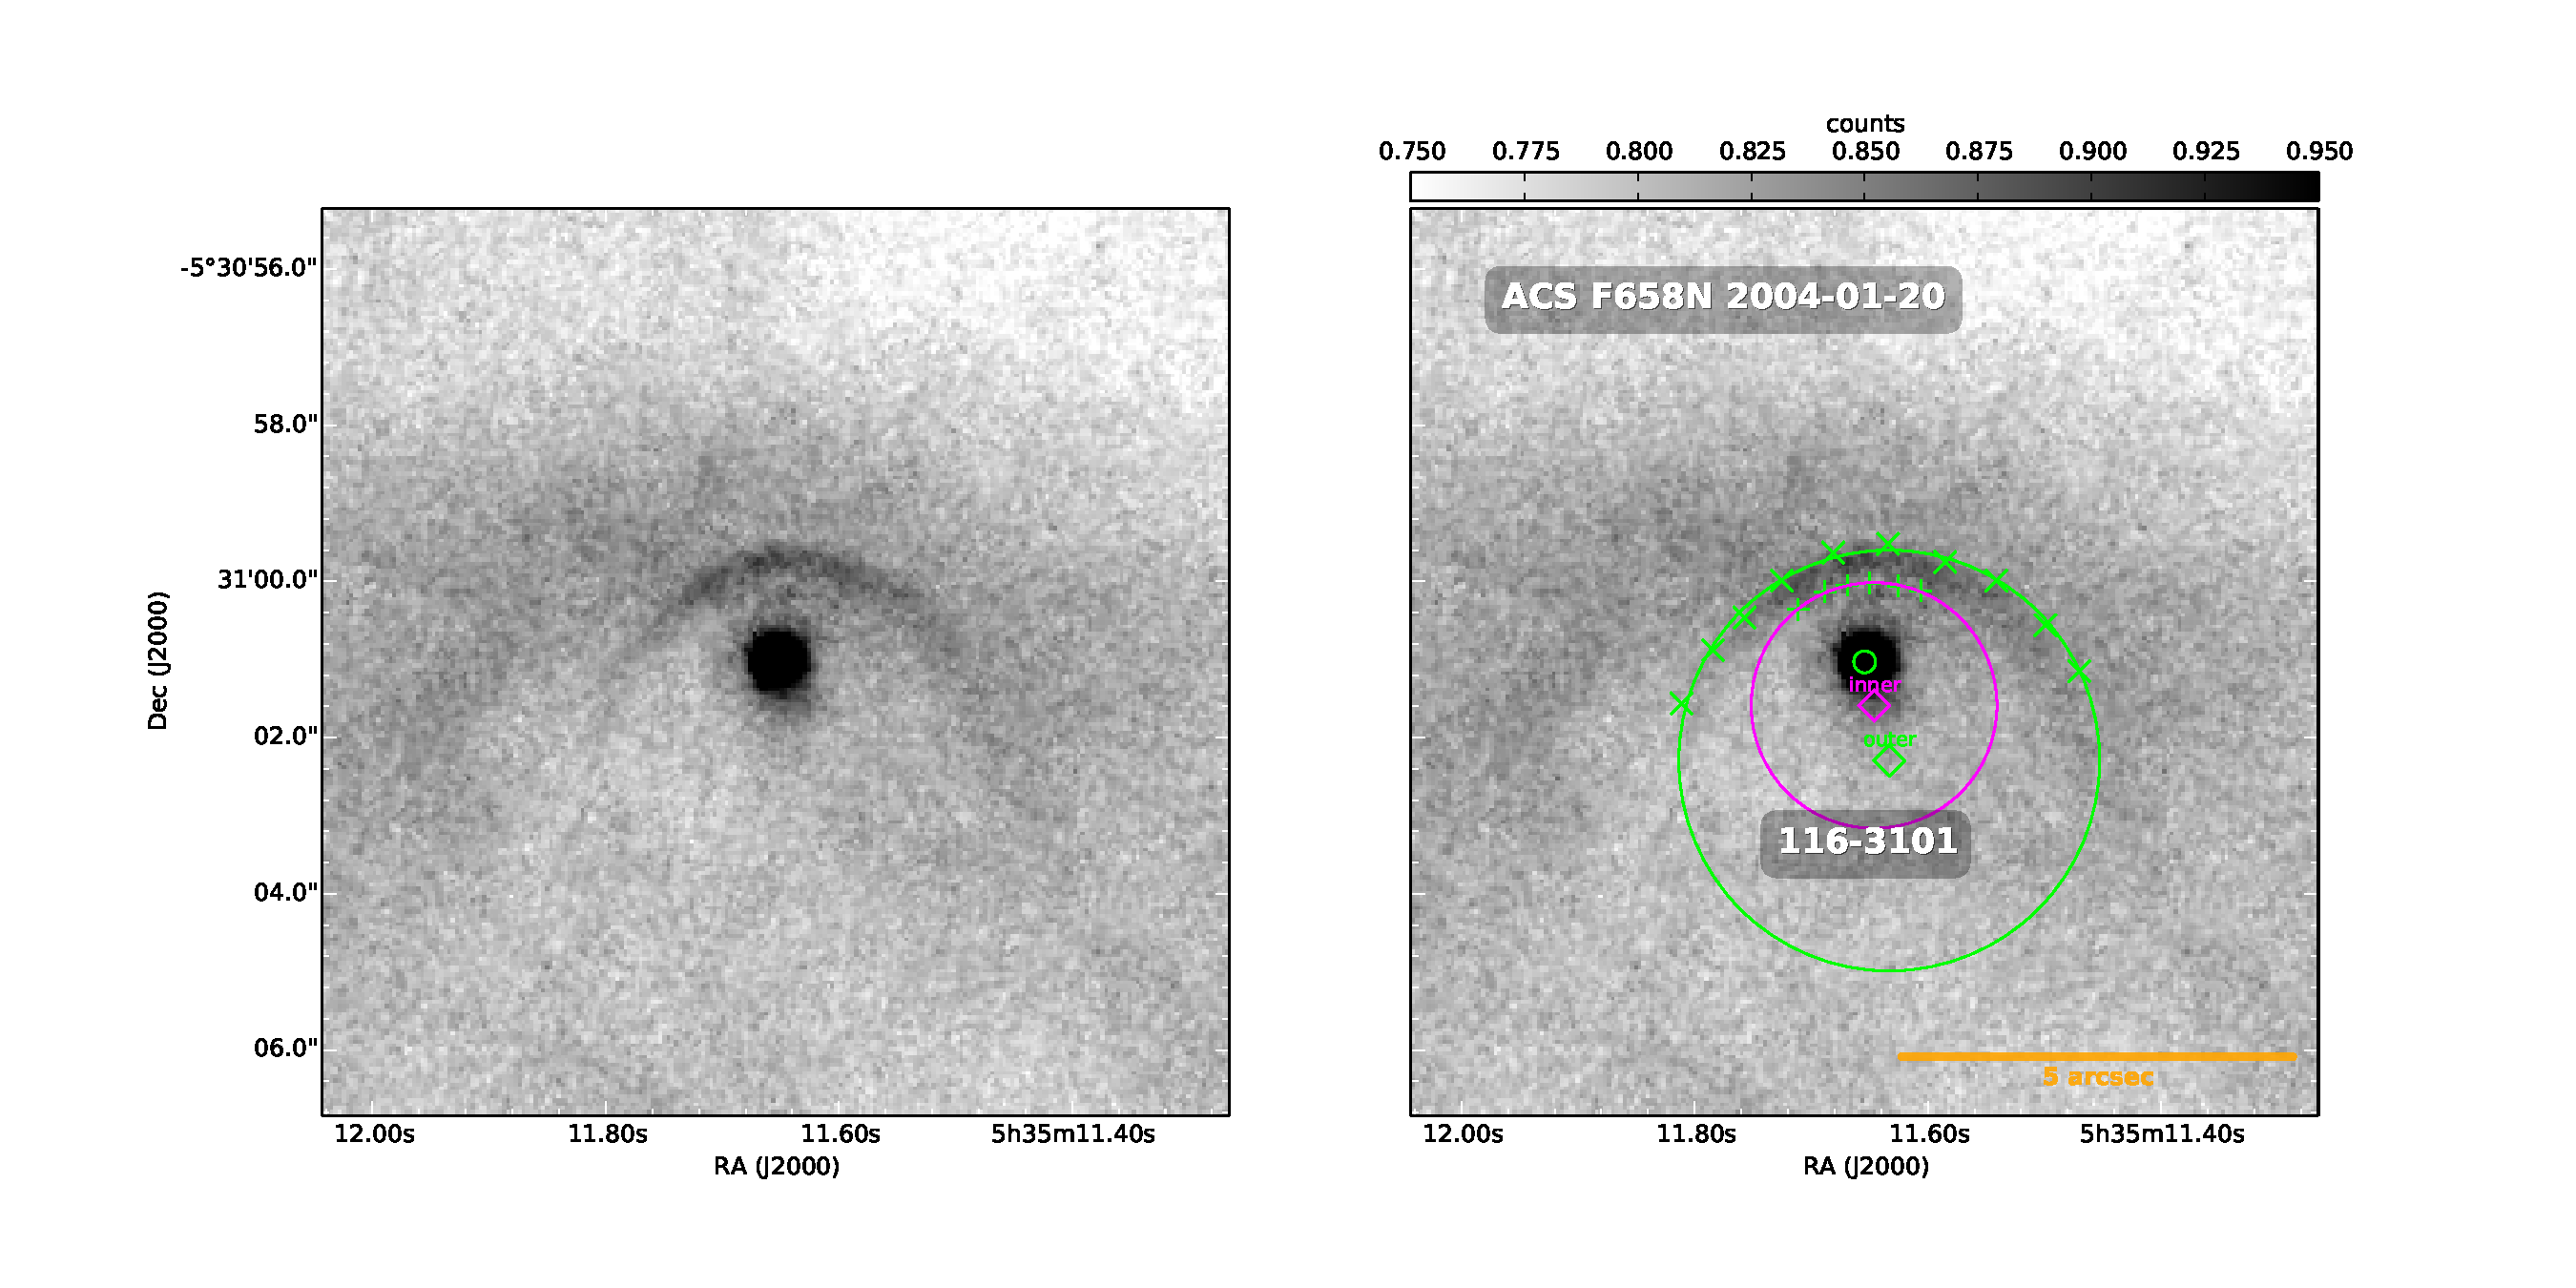
\includegraphics[width=0.5\linewidth]{./Figures/116-3101-Bally_14-images} & 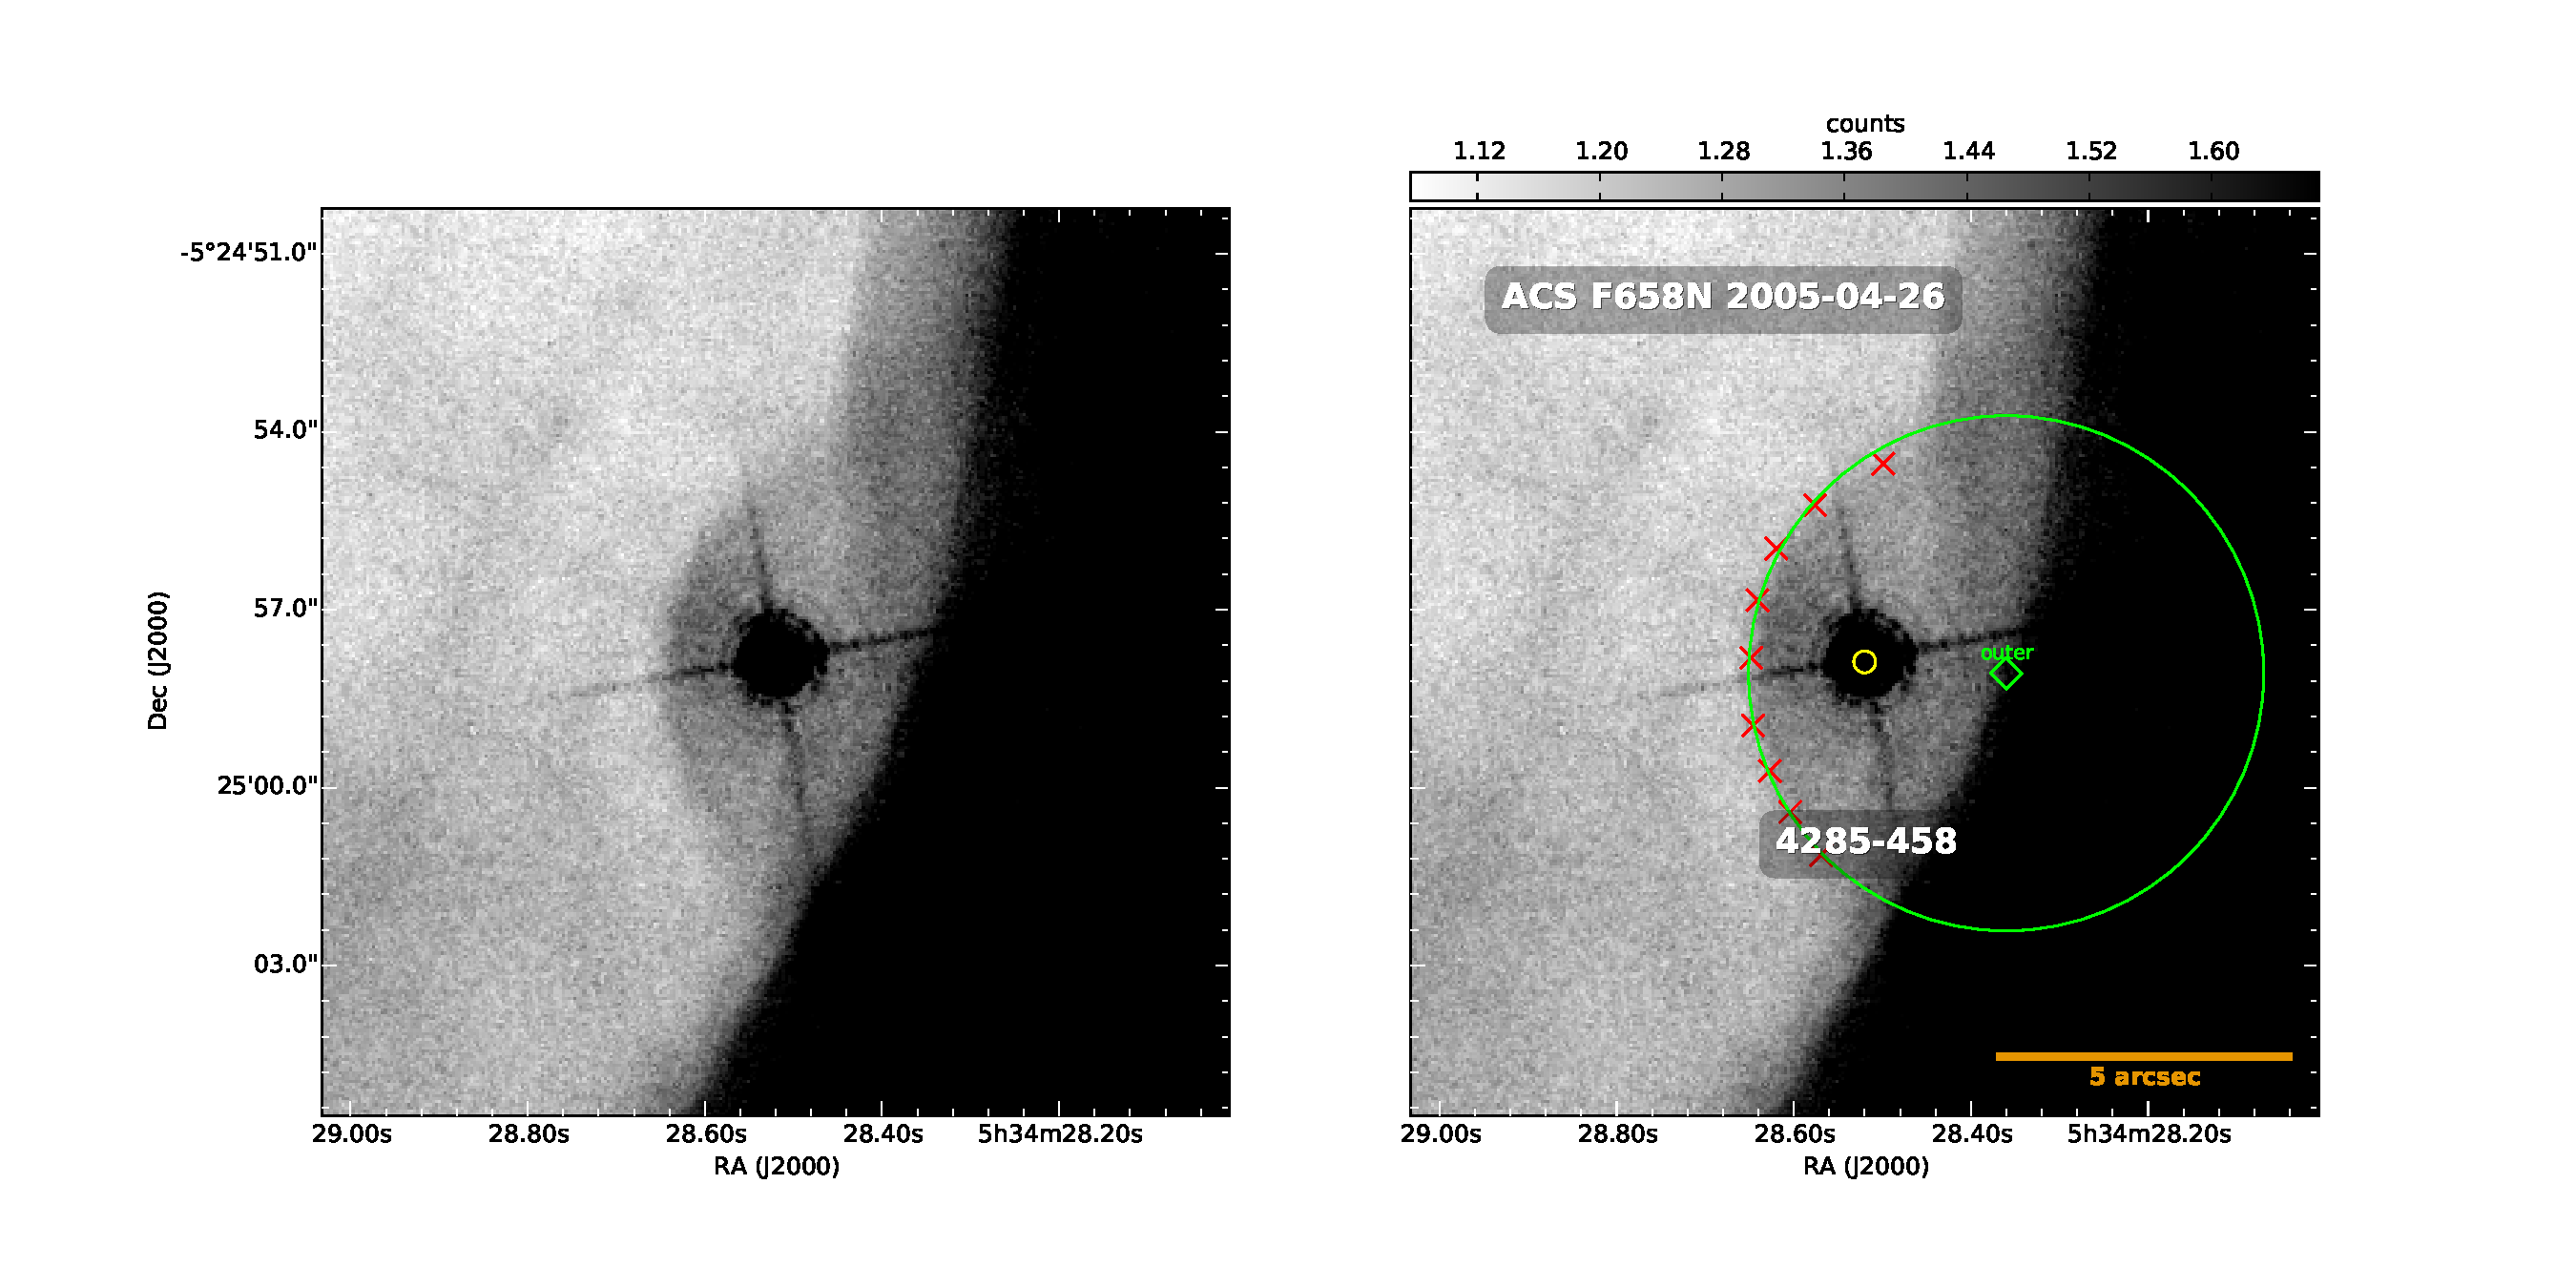
\includegraphics[width=0.5\linewidth]{./Figures/4285-458-Robberto_ACS_1r_f658n-images} \\ 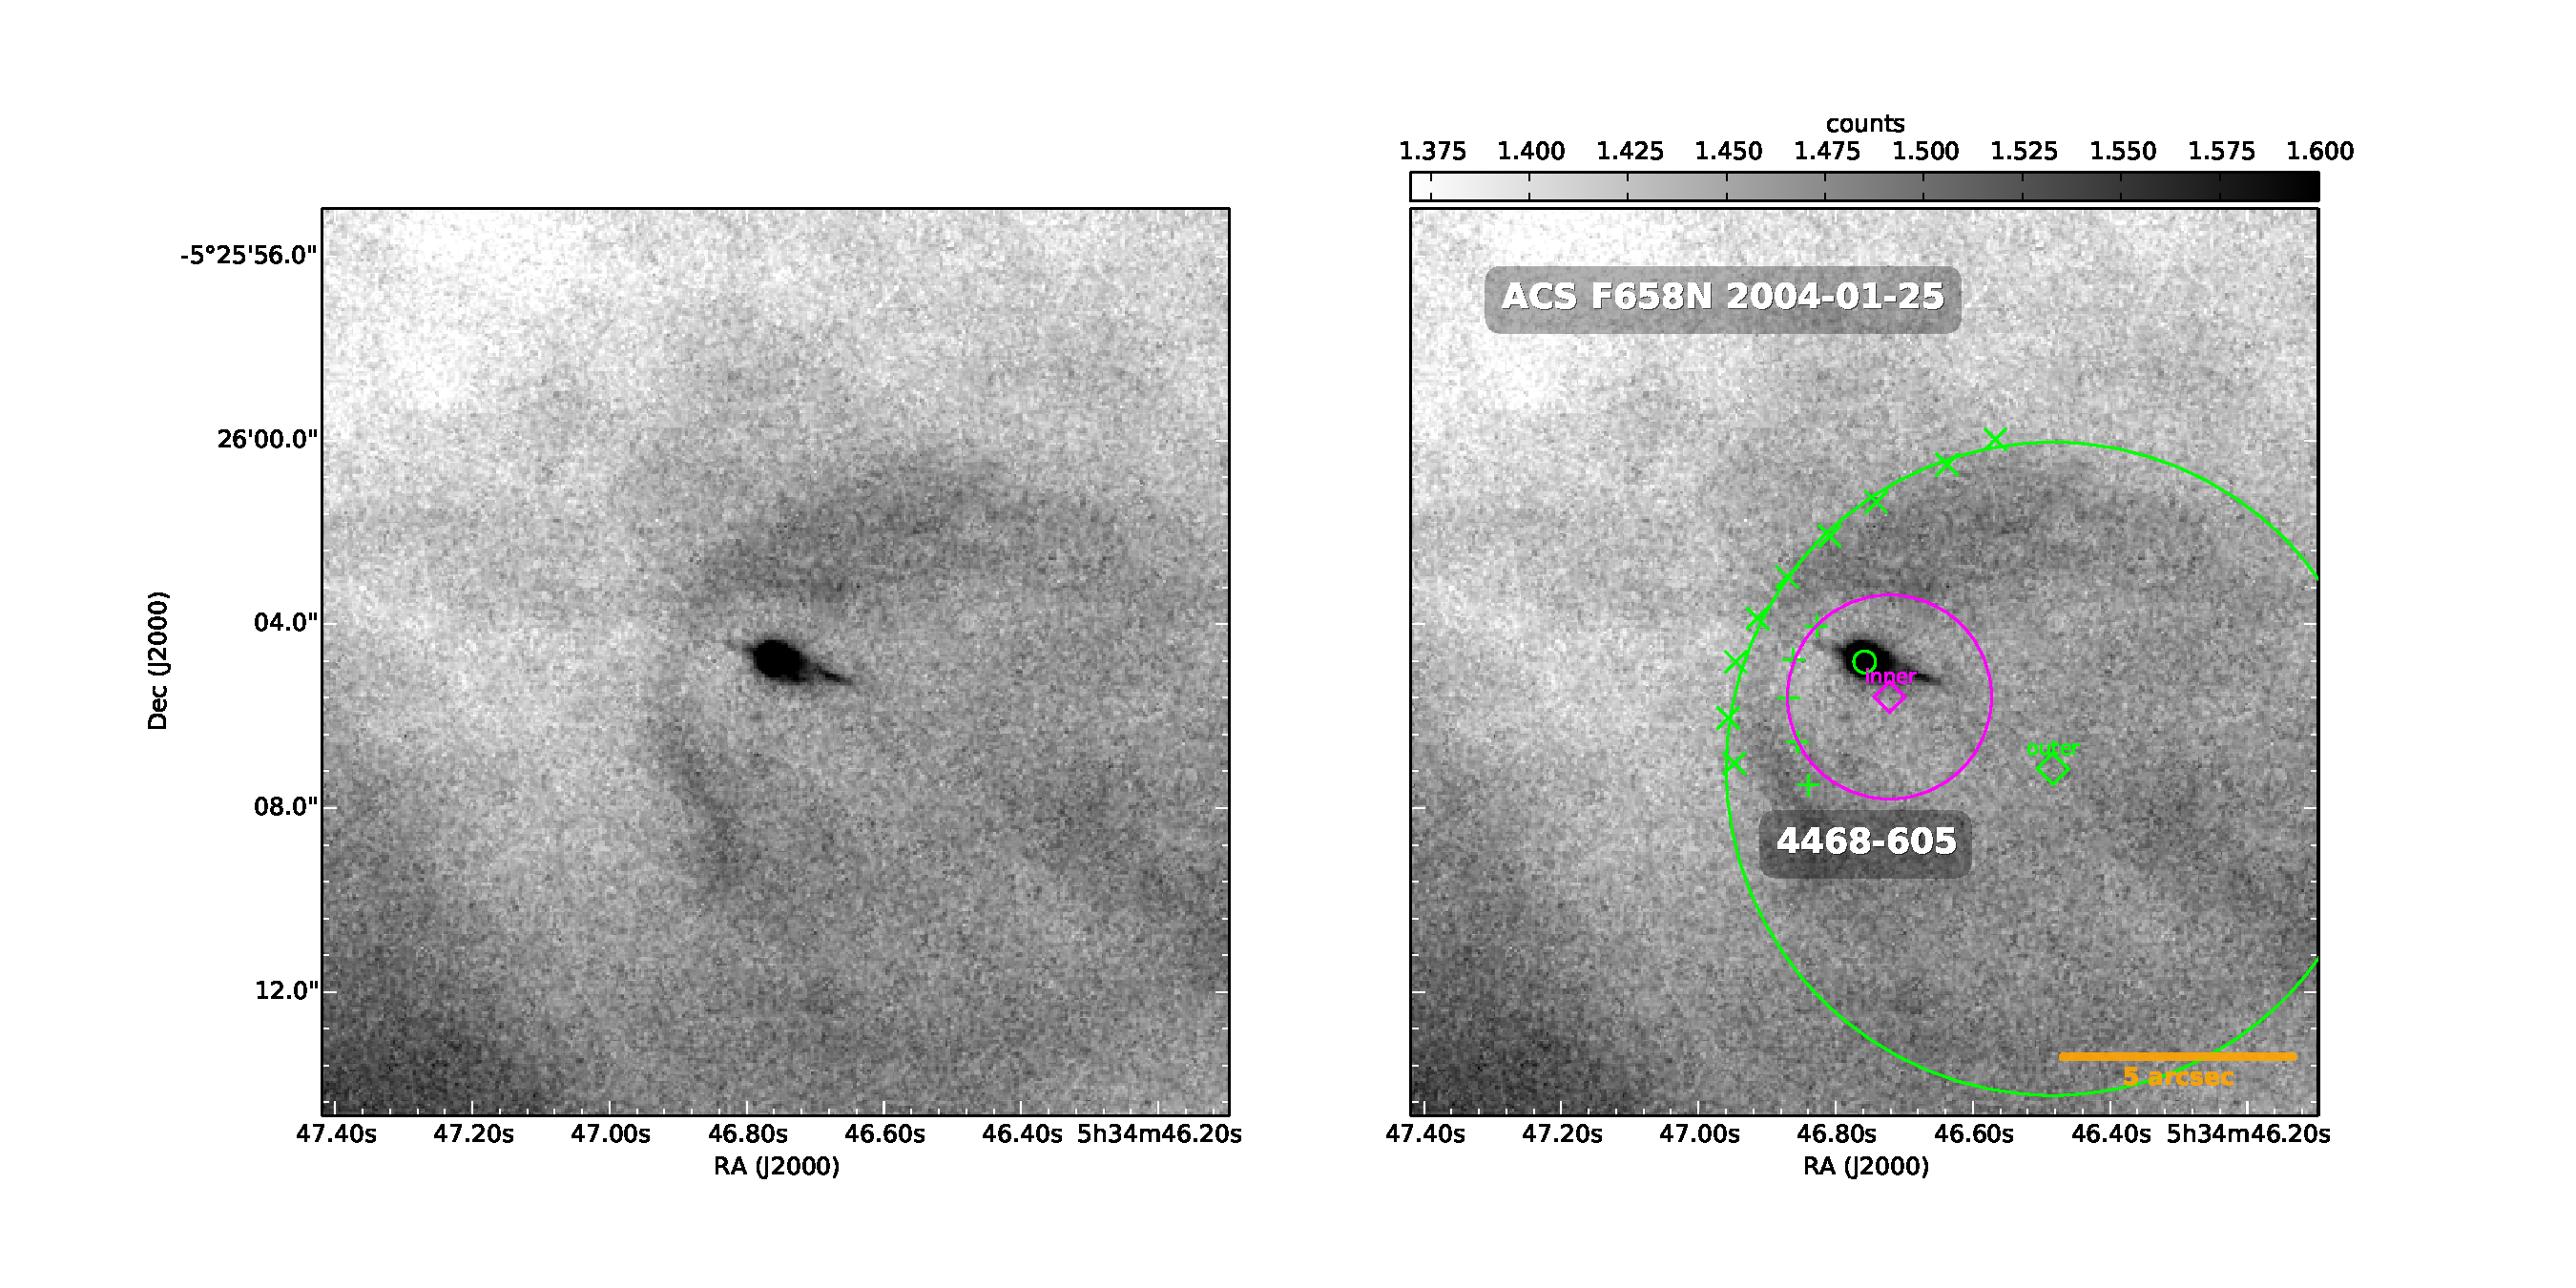
\includegraphics[width=0.5\linewidth]{./Figures/4468-605-Bally_17-images} &
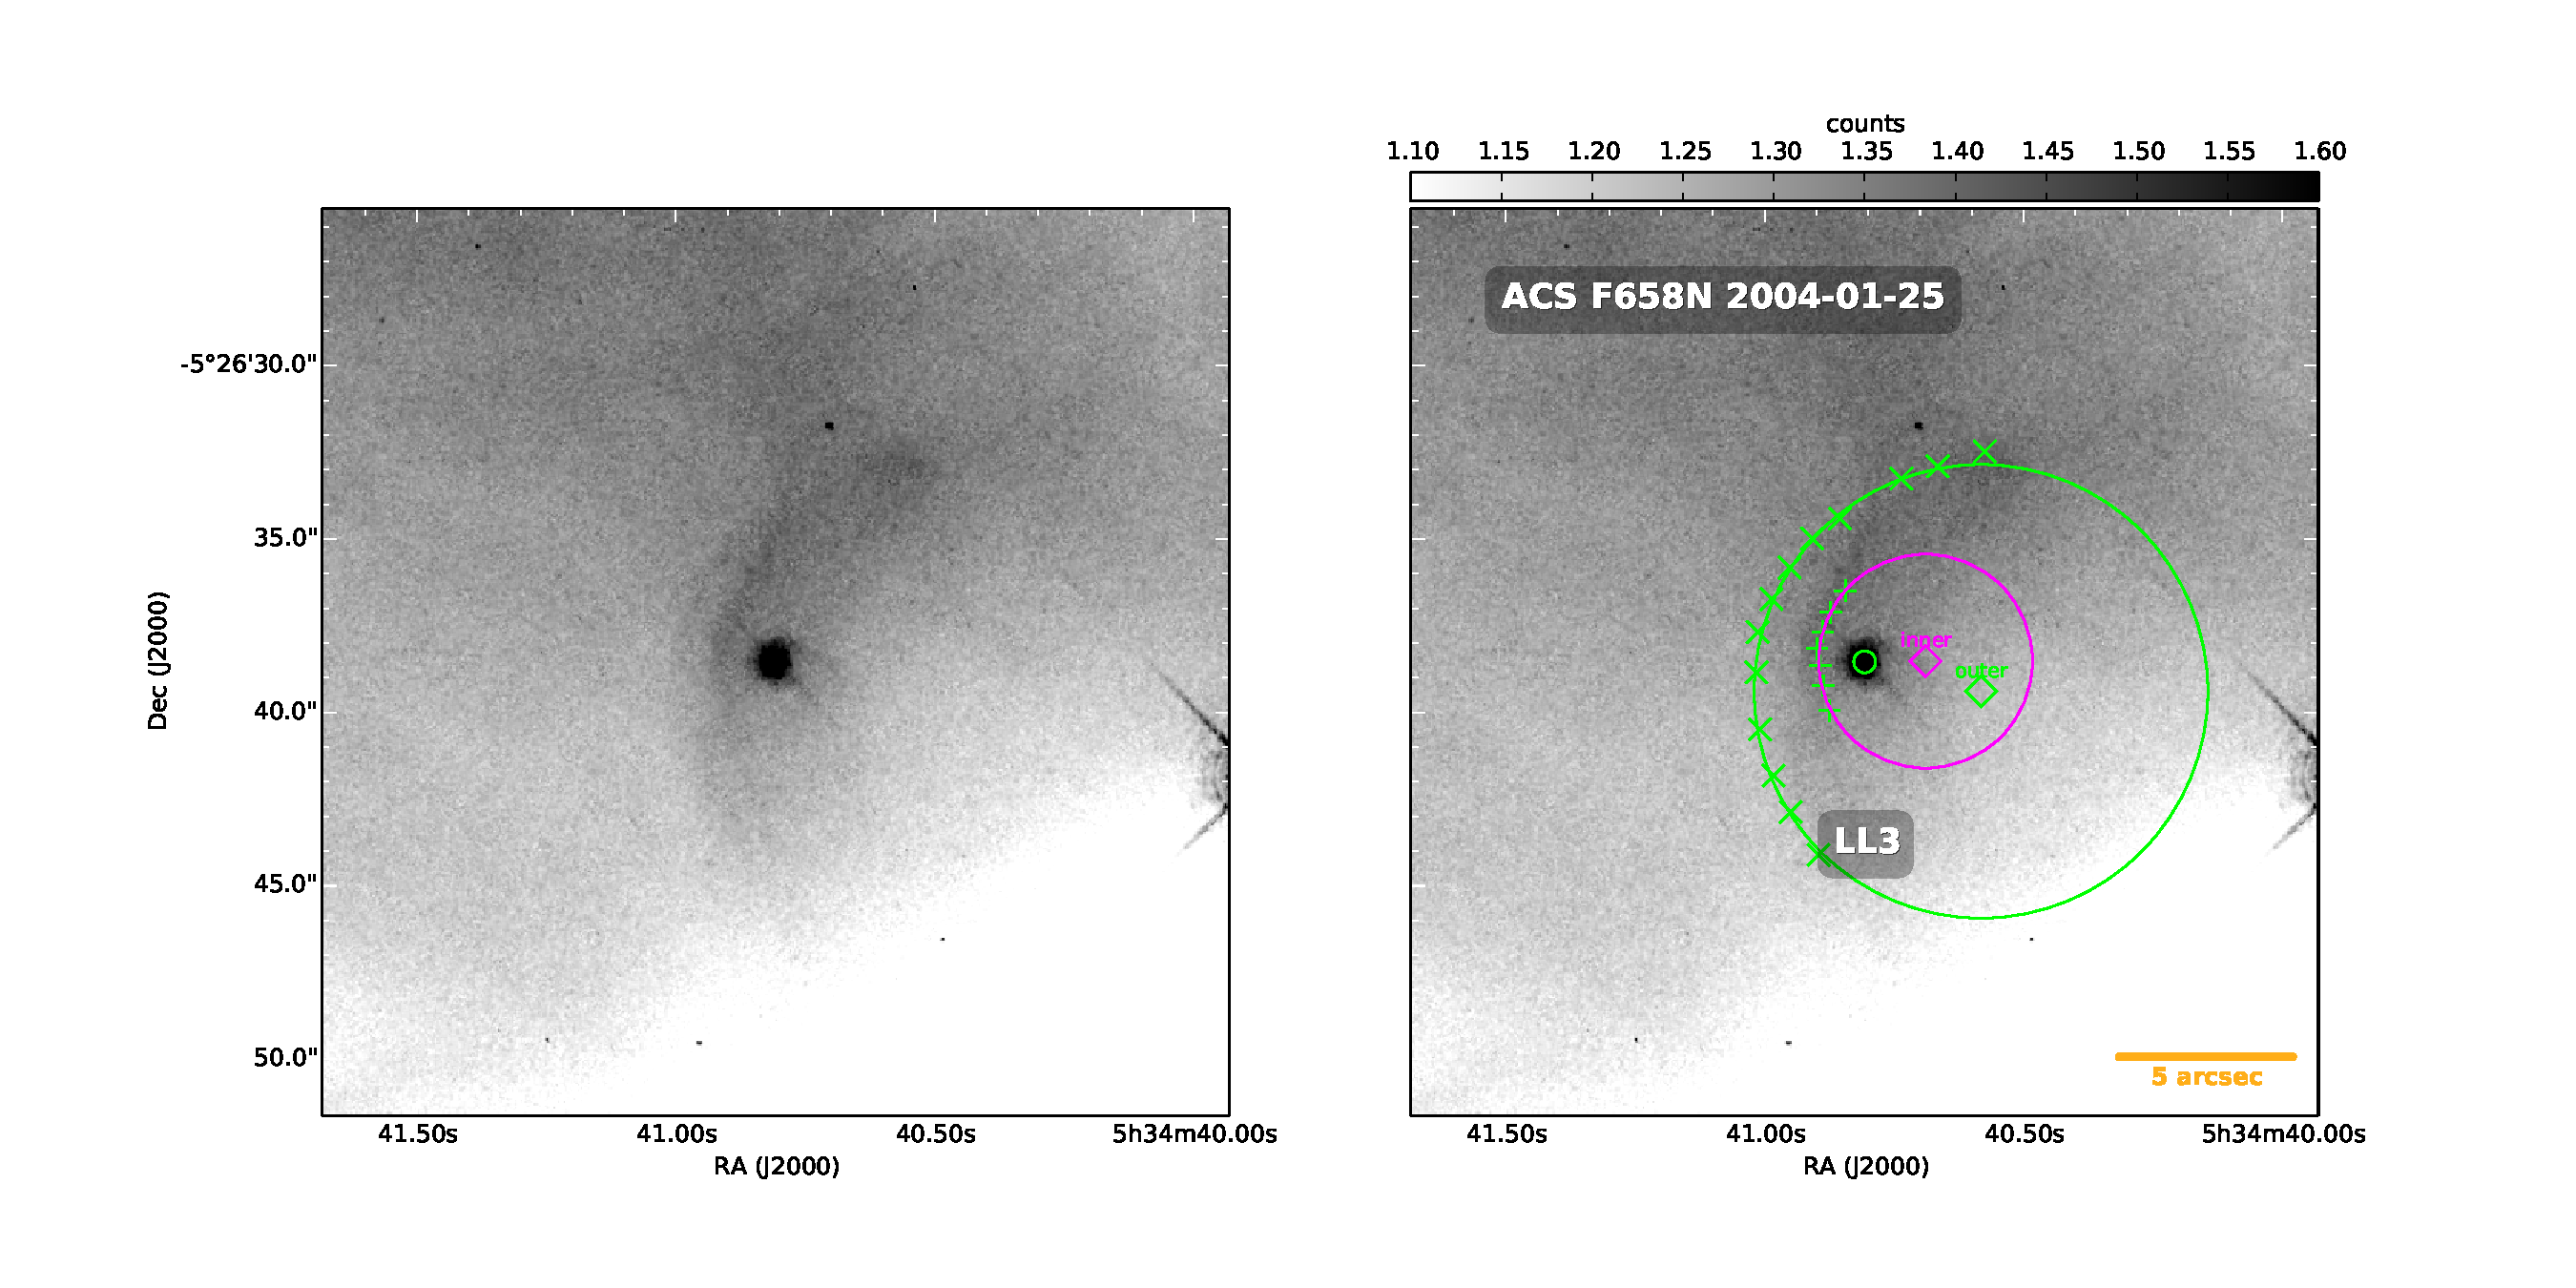
\includegraphics[width=0.5\linewidth]{./Figures/LL3-Bally_17-images}
  \end{tabular}
  \caption{}
  \label{fig:Luis-mosaic-2}
\end{figure}



\subsection{Mapa de Objetos}

A continuación en la figura \ref{fig:orion-map-LL} mostramos el mapa de los objetos del catálogo de \citet{Gutierrez-Soto:2015a} dentro de ONC.

\begin{figure}
  \centering
  \begin{tabular}{cc}
    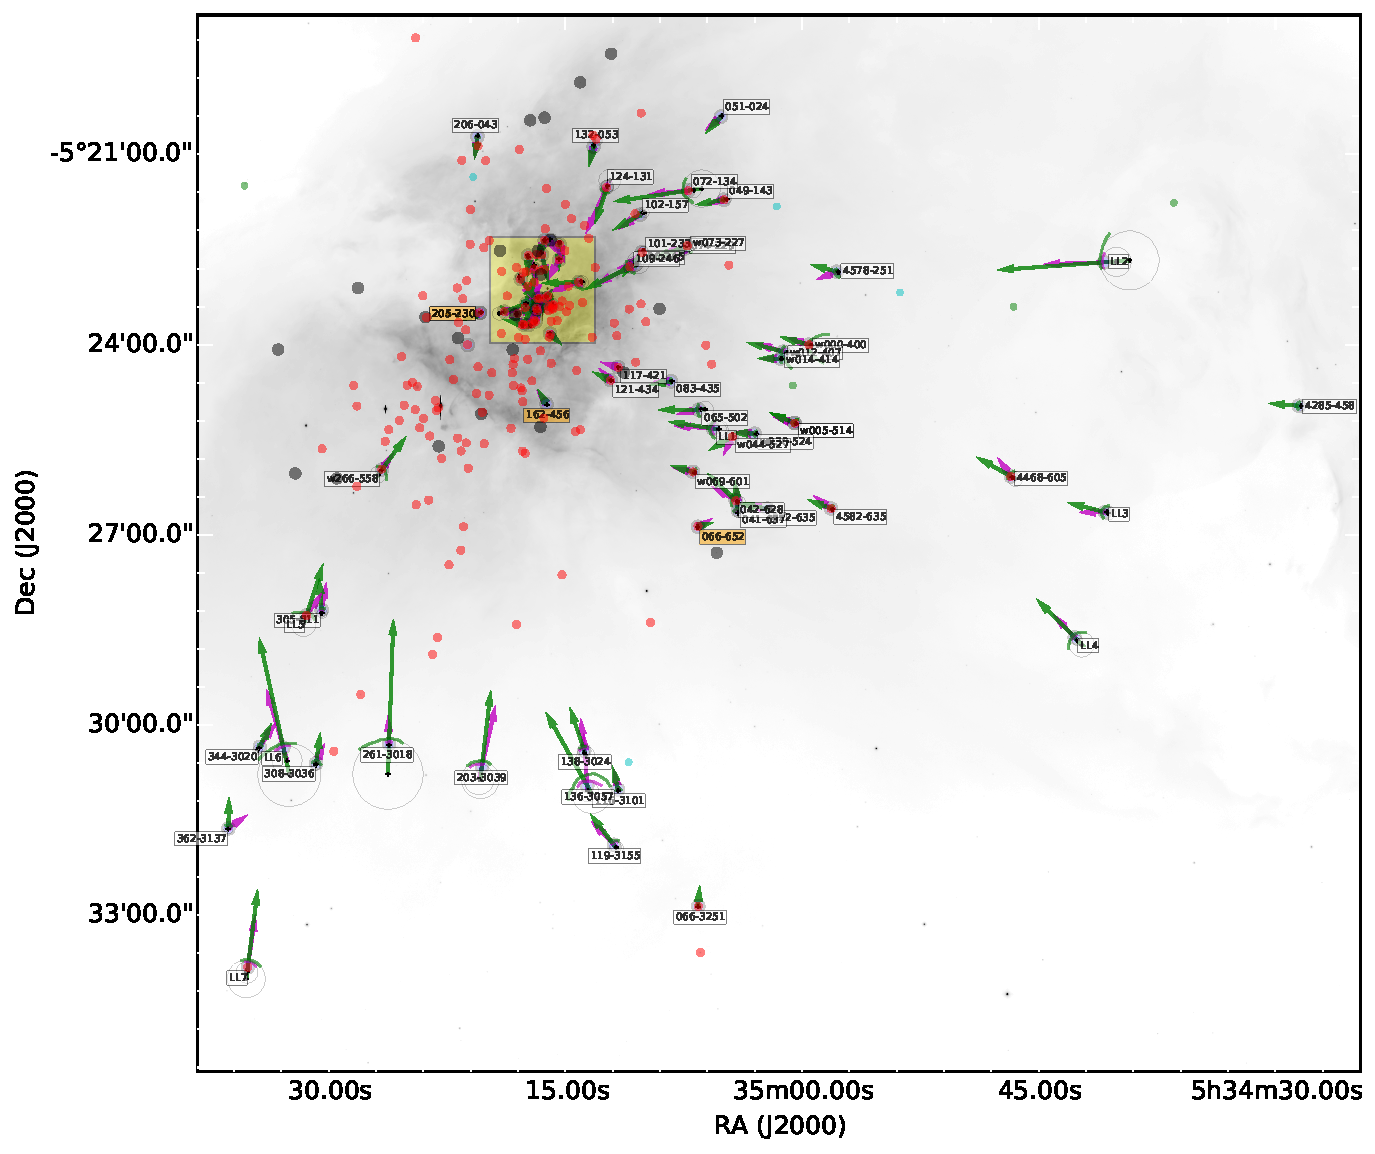
\includegraphics[width=0.5\linewidth]{./Figures/ll-pos-image-Luis} & 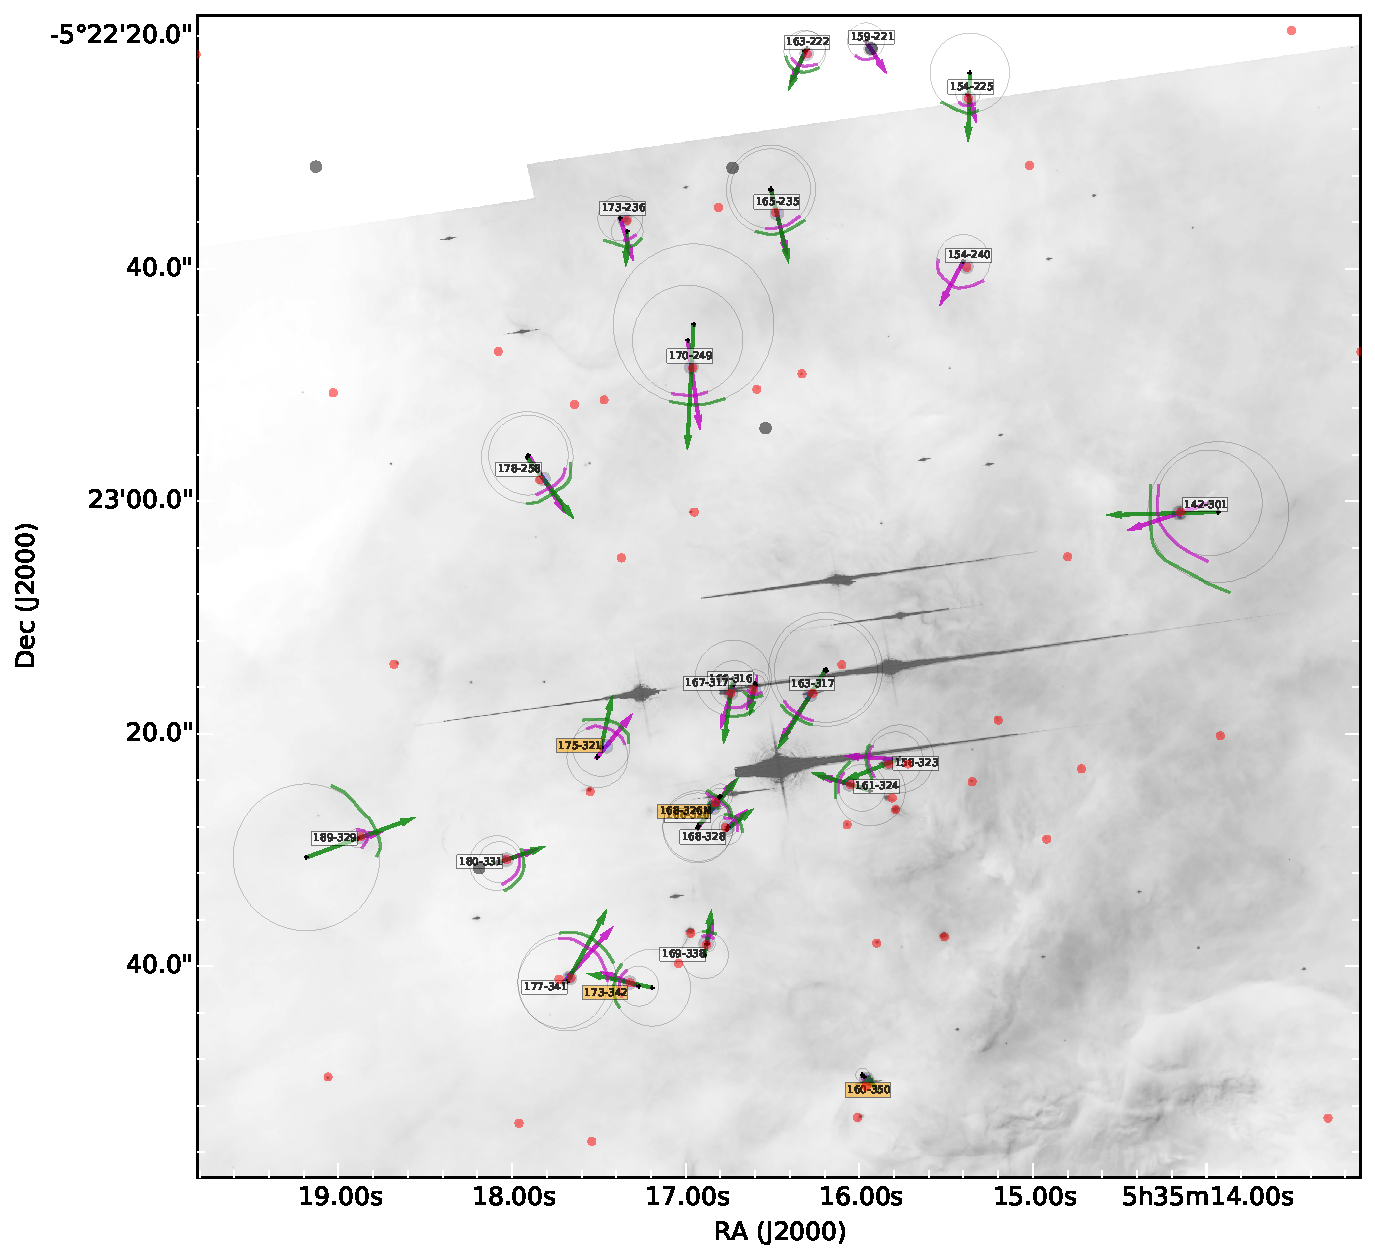
\includegraphics[width=0.46\linewidth]{./Figures/ll-pos-image-zoom-Luis}
  \end{tabular}
  \caption{Mapa de objetos del catálogo de \citet{Gutierrez-Soto:2015a} dentro de ONC. Las flechas de colores contienen la línea que une la posición del objeto central con el eje de curvatura de cada cáscara. Los puntos rojos representan objetos que no tienen un choque de proa visible. La zona marcada con el cuadrado amarillo se encuentra amplificada en el pánel derecho.}
  \label{fig:orion-map-LL}
\end{figure}


\section{Estrellas ``Errantes''}
\label{sec:runaway}

Otro tipo de choques de proa estelares ocurren cuando los vientos de estrellas \textit{errantes} (runaway stars), usualmente de tipos espectrales OB, con velocidades mayores a \SI{30}{km.s^{-1}} interactúan con el medio interestelar \citep{Kobulnicky:2016}. Estas estrellas adquieren estas velocidades cuando sufren encuentros dinámicos cercanos dentro del cúmulo donde se formaron o bien cuando forman parte de un sistema binario cerrado y uno de los miembros explota como supernova.

En la figura \ref{fig:runaway} se muestran algunos ejemplos típicos de choques de proa producidos por estrellas errantes. Los colores en cada imagen representan a la banda de \SI{24}{\mu.m} del Telescopio Espacial Spitzer, o bien la de \SI{22}{\mu.m} del catálogo WISE para el color rojo, para el color verde puede ser la banda de \SI{8}{\mu.m} de Spitzer o la de \SI{12}{\mu.m} de WISE, y al color azul le corresponde la banda de \SI{4.5}{\mu.m} de Spitzer o WISE y los objetos mostrados son, de arriba a abajo y de izquierda a derecha: $\zeta$\,Oph, AE Aur, HD136003, HD150898, HD155755 y HD143275, y por último, la flecha blanca indica la magnitud y dirección del movimiento propio de la estrella.

\begin{figure}
  \centering
  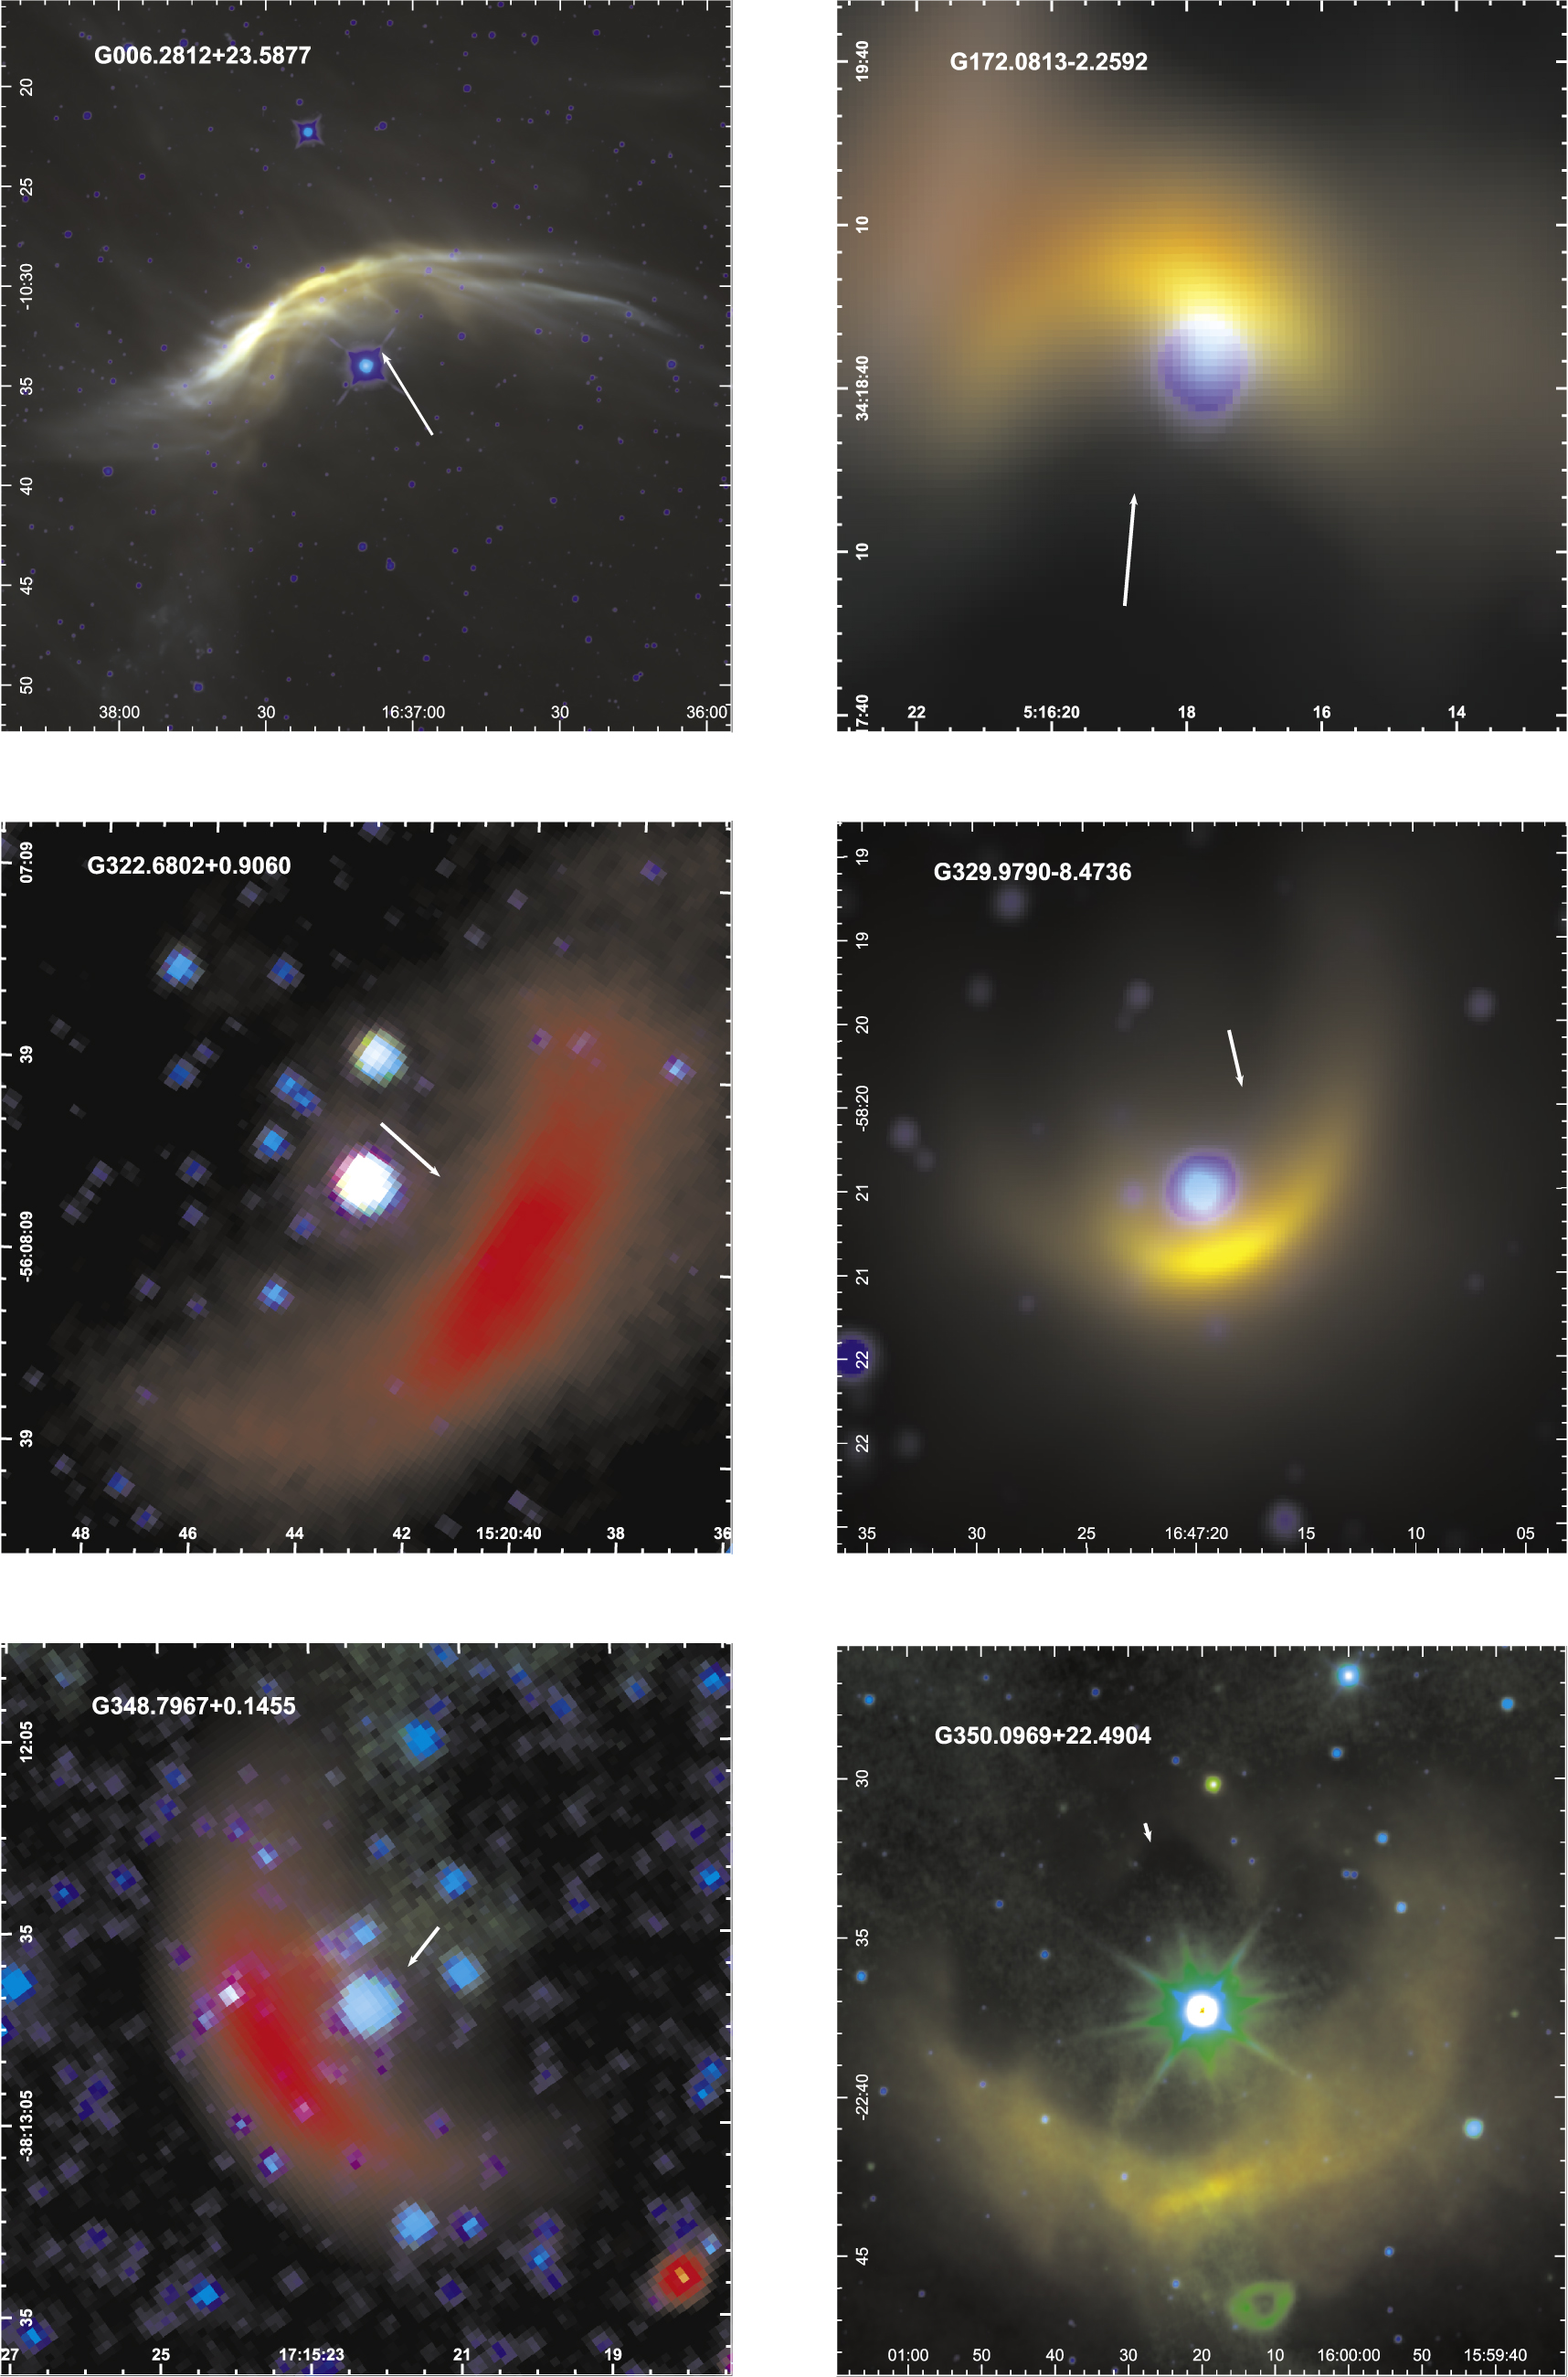
\includegraphics[width=0.7\linewidth]{./Figures/kobulnicky}
  \caption{Ejemplos de choques de proa en infrarrojo producidos por estrellas errantes, tomados por el telescopio espacial Spitzer o del catálogo WISE. Los colores representan las bandas de \SI{24}{\mu.m} de Spitzer o \SI{22}{\mu.m} de WISE (rojo), \SI{8}{\mu.m} de Spitzer o \SI{12}{\mu.m} de WISE (verde) y \SI{4.5}{\mu.m} de de Spitzer o WISE (azul). Los objetos mostrados son: $\zeta$\, Oph (G006.2812+23.5877; arriba izquierda), AE Aur (G172.0813-02.2592; arriba derecha), HD136003 (G322.6802+00.9060; centro izquierda), HD150898 (G329.9790-08.4736; centro derecha), HD155755 (G348.7967+00.1455; abajo izquierda) y HD143275 (G350.0969+22.4904; abajo derecha). La magnitud y dirección del movimiento propio se muestra con las flechas blancas \citep{Kobulnicky:2016}.}
  \label{fig:runaway}
\end{figure}

\section{Estrellas AGB y Supergigantes Rojas}
\label{sec:AGBs}
Otro tipo de choques de proa estelares se forma cuando estrellas en sus fases evolutivas finales, tales como estrellas AGB y supergigantes rojas pierden material a través de fuertes vientos que producen choques al interaccionar con el Medio Interestelar \citep{Cox:2012}.

En la figura  \ref{fig:fermata} se muestran ejemplos de estrellas AGB y supergigantes en infrarrojo lejano que forman parte del programa MESS (Mass-loss of Evolved StarS, \citet{Groenewegen:2011}) que utilizan el instrumento PACS (Photodetector Array Camera Spectrometer), donde se usan los filtros de \SI{70}{\mu.m} y \SI{160}{\mu.m}, y que muestran choques tipo ``fermata''. Otras formas que se observan son tipo ``ojos'', ``anillos'' e ``irregulares'' (ver tabla \ref{tab:morphology-AGB}).

\begin{figure}
  \centering
  \includegraphics[width=0.5\linewidth]{./Figures/Cox-fermata}
  \caption{Interacciones tipo ``fermata'' de los objetos R\,Scl, NML\,Tau, W\,Ori, W\,Pic y $\alpha$\,Ori tomadas con PACS en los filtros de \SI{70}{\mu.m} (izquierda) y \SI{160}{\mu.m} (derecha). La barra blanca mide 1' en la imagen, así como su respectivo tamaño físico. En todos los páneles el norte se ubica hacia arriba y el este a la izquierda. La línea negra indica la velocidad y dirección de la velocidad espacial de la estrella, adoptando una escala tal que \SI{1}{km.s} corresponde a 1'' en la imagen \citep{Cox:2012}. Nota adicional. R\,Scl tiene una cáscara esférica interna no visible en la imagen.}
  \label{fig:fermata}
\end{figure}

\begin{table}
  \centering
  \begin{tabular}{llc}
    \toprule
    Clase & Descripción & Forma \\
    \midrule
    I & Fermata & 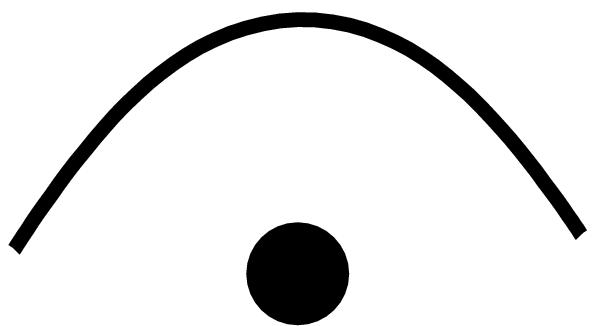
\includegraphics[scale=0.03]{./Figures/fermata} \\
    II & Ojos   & 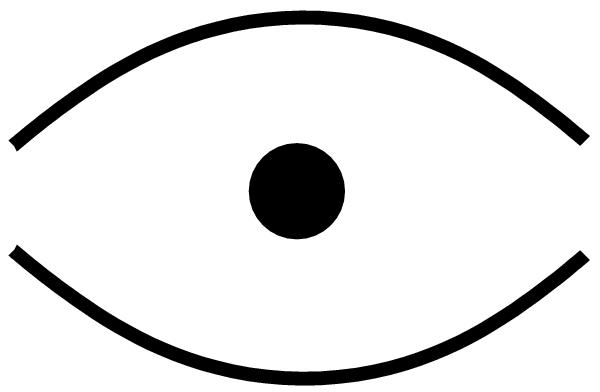
\includegraphics[scale=0.03]{./Figures/eyes} \\
    III & Anillos & 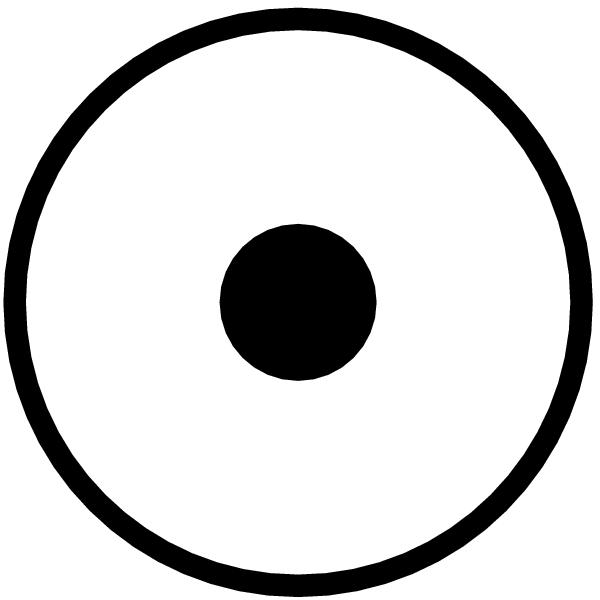
\includegraphics[scale=0.02]{./Figures/ring} \\
    IV & Irregulares & \\
    \bottomrule
  \end{tabular}
  \caption{Clasificación morfológica de choques de proa estelares de estrellas AGB y supergigantes \citep{Cox:2012}.}
  \label{tab:morphology-AGB}
\end{table}


%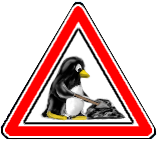
\includegraphics[width=0.1\linewidth]{./Figures/tux-development}
